\documentclass[en,t]{sdqbeamer}
%\documentclass[c]{sdqbeamer}

\usepackage{listings}
\usepackage{graphicx}
\usepackage{tabularx}
\usepackage{multirow}
\usepackage{multicol}
\usepackage{tabulary}
\usepackage{colortbl}
\usepackage{tikzsymbols}
\usepackage{tikz}
\usepackage{booktabs}
\usetikzlibrary{positioning,fit,shapes}
\usepackage[lined,linesnumbered,ruled,noend]{algorithm2e}
\usepackage{bm}

\hypersetup{
	colorlinks=true,
	urlcolor=kit-orange
}

% set sdqbeamer options
\titleimage{blender-render}
\groupname{Algorithm Engineering}
\grouplogo{ae}
%\selectlanguage{english}


\usepackage[backend=biber,style=numeric-comp,sorting=none]{biblatex}
\addbibresource{references.bib}

% define title etc.pp.
\title[SAT Solving]{Practical SAT Solving}
\subtitle{Lecture 11: Application Highlights}
\author{\underline{Markus Iser}, Dominik Schreiber, Tom\'a\v{s} Balyo}
\date{July 1, 2024}

% Existing KIT colors: kit-green, kit-blue, kit-red, kit-gray, kit-orange, kit-lightgreen, kit-brown, kit-purple, kit-cyan
% configure appearance
\setbeamercolor{block title}{bg=kit-blue}
\setbeamercolor{block body}{bg=kit-blue!10}
\setbeamercolor{block title example}{bg=kit-orange}
\setbeamercolor{block body example}{bg=kit-orange!10}
\setbeamertemplate{itemize item}{\color{kit-gray}\textbullet}
\setbeamertemplate{itemize subitem}{\color{kit-gray}\textbullet}
\setbeamercolor{item projected}{bg=kit-gray, fg=kit-gray}
\renewcommand{\insertnavigation}[1]{} % remove navigation bar

% define commands
\definecolor{myblue}{HTML}{0D3B66}
\definecolor{myred}{HTML}{6E0E0A}
\definecolor{mypink}{HTML}{F7B2B7}

\newcommand{\vars}[1]{\textsf{vars} (#1)}
\newcommand{\lits}[1]{\textsf{lits} (#1)}
\newcommand{\clss}[1]{\textsf{clss} (#1)}

\newcommand{\highl}[1]{\textcolor{myblue}{#1}}
\newcommand{\highlo}[1]{\textcolor{myred}{#1}}
\newcommand{\highlow}[1]{\textcolor{mypink}{#1}}

% Extra column types for tabularx
\newcolumntype{C}{>{\centering\arraybackslash}X}
\newcolumntype{L}{>{\raggedright\arraybackslash}X}
\newcolumntype{R}{>{\raggedleft\arraybackslash}X}

\newcommand{\setcolsep}[1]{\setlength{\tabcolsep}{#1}}
\newcommand{\setrowsep}[1]{\renewcommand{\arraystretch}{#1}}

% Definitions for the Tseitin transformation
\newcommand{\true}{\ensuremath{\mathit{True}}}
\newcommand{\false}{\ensuremath{\mathit{False}}}
\newcommand{\allvars}{\ensuremath{\mathcal{V}}}
\newcommand{\tseitin}[1]{\ensuremath{\mathcal{T}(#1)}}
\newcommand{\tseitinRec}[2]{\ensuremath{\mathcal{T}^{#2}(#1)}}
\newcommand{\tseitinSym}[1]{\ensuremath{\mathcal{T}_\mathsf{lit}(#1)}}
\newcommand{\tseitinDef}[2]{\ensuremath{\mathcal{T}_\mathsf{def}^{#2}(#1)}}
\newcommand{\hcancel}[2][black]{\setbox0=\hbox{$#2$}\rlap{\raisebox{.45\ht0}{\textcolor{#1}{\rule{\wd0}{1pt}}}}#2} 
\newcommand{\sateq}{\mathrel{\overset{\makebox[0pt]{\mbox{\normalfont\tiny\sffamily SAT}}}{=}}}

\newcommand{\enc}{\ensuremath{\mathcal{E}}} % encoding

% exercise commands
\newcommand{\exhead}[3]{
\hrule~\\[1ex]\noindent
{\bf Practical SAT Solving} (ST 2024) \hfill \fbox{Assignment #1} \\[1ex]
Markus Iser, Dominik Schreiber, Tom\'a\v{s} Balyo\\[1ex]
Algorithm Engineering (KIT) \hfill #2 -- #3\\
\hrule
\thispagestyle{empty}
}


\renewcommand{\highl}[1]{\textcolor{kit-blue}{#1}}
\renewcommand{\highlo}[1]{\textcolor{kit-orange}{#1}}
\newcommand{\unimp}[1]{\textcolor{gray}{#1}}

% Redefine `\rowcolor` to allow a beamer overlay specifier
% New syntax: \rewcolor<overlay>[color model]{color}[left overhang][right overhang]
\makeatletter
% Open `\noalign` and check for overlay specification:
\def\rowcolor{\noalign{\ifnum0=`}\fi\bmr@rowcolor}
\newcommand<>{\bmr@rowcolor}{%
    \alt#1%
        {\global\let\CT@do@color\CT@@do@color\@ifnextchar[\CT@rowa\CT@rowb}% Rest of original `\rowcolor`
        {\ifnum0=`{\fi}\@gooble@rowcolor}% End `\noalign` and gobble all arguments of `\rowcolor`.
}
% Gobble all normal arguments of `\rowcolor`:
\newcommand{\@gooble@rowcolor}[2][]{\@gooble@rowcolor@}
\newcommand{\@gooble@rowcolor@}[1][]{\@gooble@rowcolor@@}
\newcommand{\@gooble@rowcolor@@}[1][]{\ignorespaces}
\makeatother

% Redefine '\cellcolor' for beamer overlay use
\renewcommand<>\cellcolor[1]{\only#2{\beameroriginal\cellcolor{#1}}}

\begin{document}
\begin{frame}
	\thispagestyle{empty}
	\titlepage
\end{frame}


\begin{frame}{Why consider the Application View? (1/2)}
	
	\vspace*{-2mm}
	\centering
	\small
	\begin{tabular}{llll}
		\toprule
		\multicolumn{2}{l}{\textbf{Result, instance family}} & \textbf{1st author} & \textbf{Speedups of \textsc{MallobSat} over \textsc{Kissat-MAB\_HyWalk}} \\
		\midrule
		% "Kakuro"; very large, sharing long clauses
		SAT & Hypertree decomposition 					 & Schidler & 3, 5, 5, 5, 5, 7, 8, 9, 12, 13 \\
		% lowest speedups are where the seq. solver is reasonably fast (100s)
		SAT & Hamilton circle 							 & Heule & 4, 4, 7, 11, 17, 20, 21, 22, 24, 31, 33, 36, 42 \\
		% very large, sharing long clauses
		SAT & Tree decomposition 						 & Ehlers & 5, 7, 87 \\
		% sharing pretty long clauses; pretty large inputs which the seq. solver solves reasonably quickly
		UNSAT & Cellular automatons 						 & Chowdhury & 5, 8, 8, 9, 9, 10, 22, 22, 66 \\
		\multicolumn{4}{c}{\vdots} \\[1mm]
		% Only clauses of length <= 4 shared
		UNSAT & Relativized pidgeon hole				 & Elffers & 277, 542, 638 \\
		UNSAT & Bioinformatics 							 & Bonet & 292, 717 \\
		UNSAT & Balanced random 					 & Spence & 321, 388 \\
		% ONLY sharing unit clauses for two highest speedups!
		SAT & Sum of three cubes 					 & Riveros & 384, 509, 1018, 3345 \\
		\unimp{SAT} & \unimp{Circuit multiplication} & \unimp{Shunyang} & \unimp{17, 31, 32, 62, 105, 119, 213, 254, 393, 741, 746, 1401, 2650} \\
		% heavy use of cardinality constraints - Probably Lingeling. Highest speedups: solved in <1s
		\unimp{UNSAT} & \unimp{Perfect matchings} 		 & \unimp{Reeves} & \unimp{119, 413, 12\,439, 108\,593, 217\,099} \\
		\bottomrule
	\end{tabular}
	
	\vspace*{3mm}
	\unimp{\small
		3072 cores (128 machines) of SuperMUC-NG\ \ $\cdot$\ \ 400 problems from Int. SAT Competition 2021\\
		Only instances with seq.\ time $\geq 60\,$s\ \ $\cdot$\ \ Only families with $\geq 2$ instances
	}
\end{frame}

\begin{frame}{Why consider the Application View? (2/2)}
	\begin{itemize}
		\item Perform \highl{sound \textbf{algorithm engineering}} with \highlo{realistic applications} in the loop
		\item Understand \highl{application-specific solver behavior}, needs, shortcomings
		\item Advance the \highl{positive feedback loop between solvers and applications}
	\end{itemize}
	
	\vspace*{3mm}
	%\centering
	\hspace*{2cm}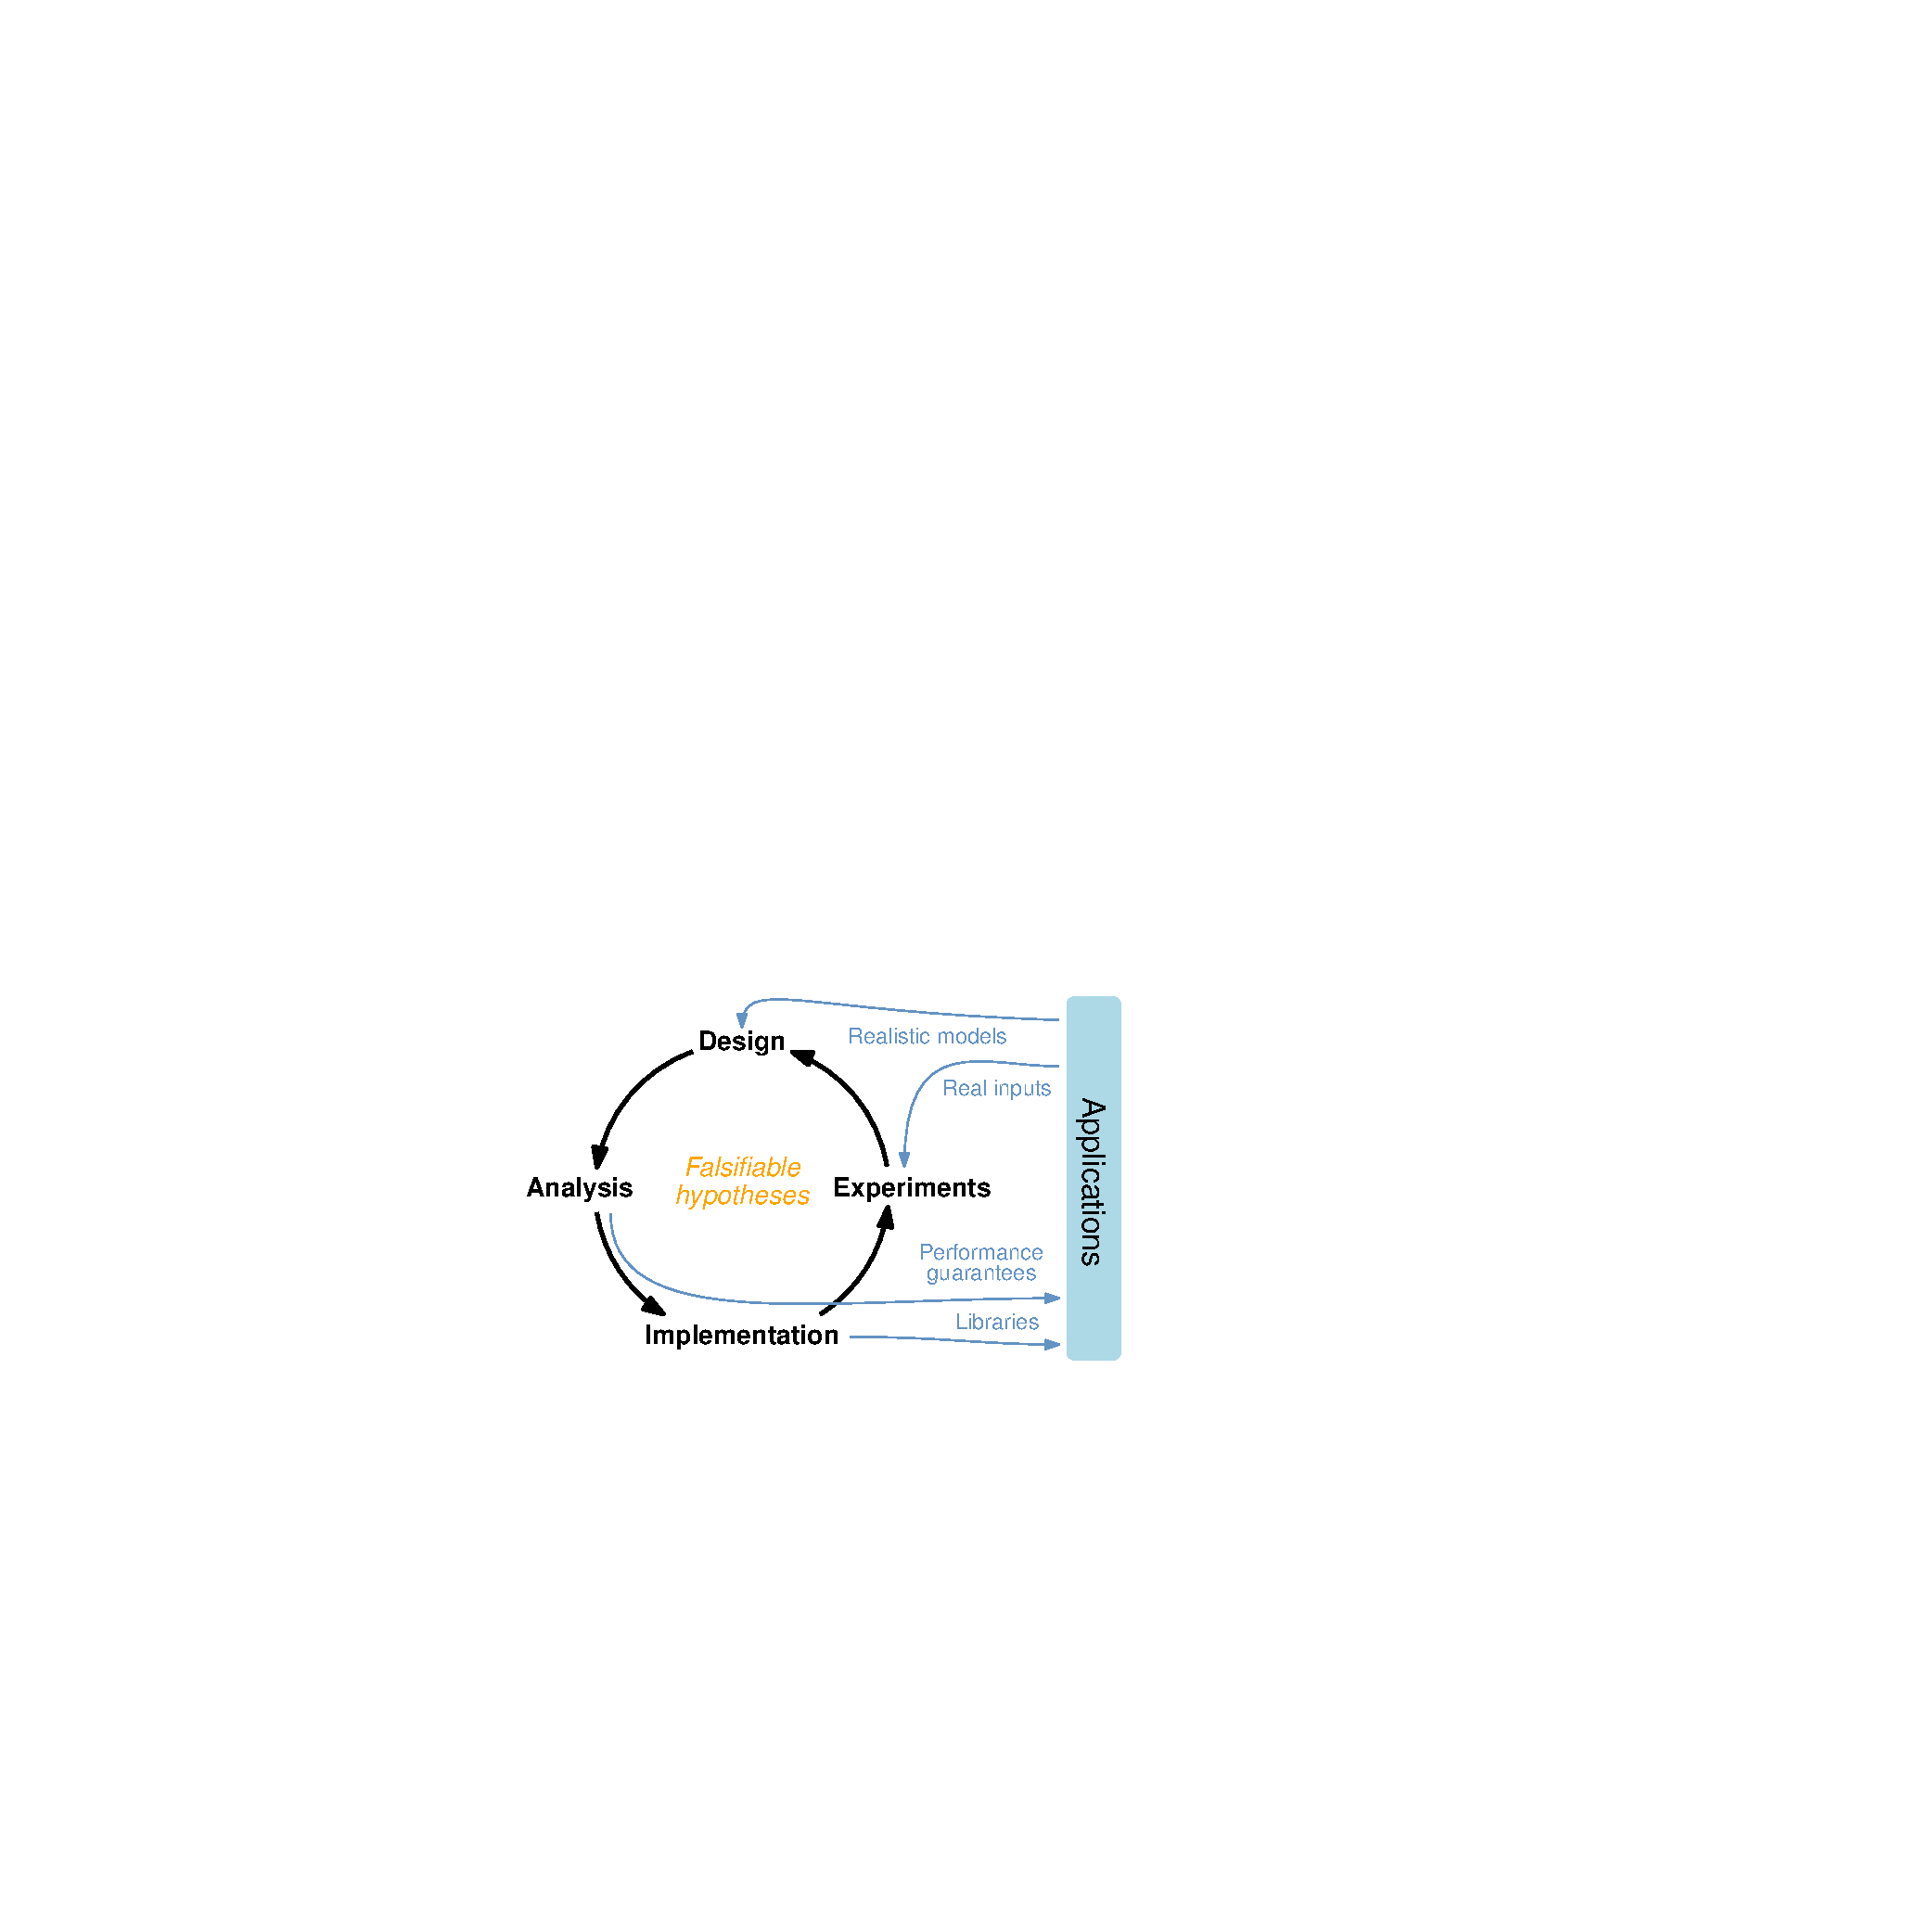
\includegraphics[width=0.5\textwidth]{figures/l11/algorithm-engineering.pdf}
\end{frame}

\begin{frame}{SAT Competition Benchmarks -- ``Real'' Applications?}
	\begin{minipage}{0.73\textwidth}
		\centering
		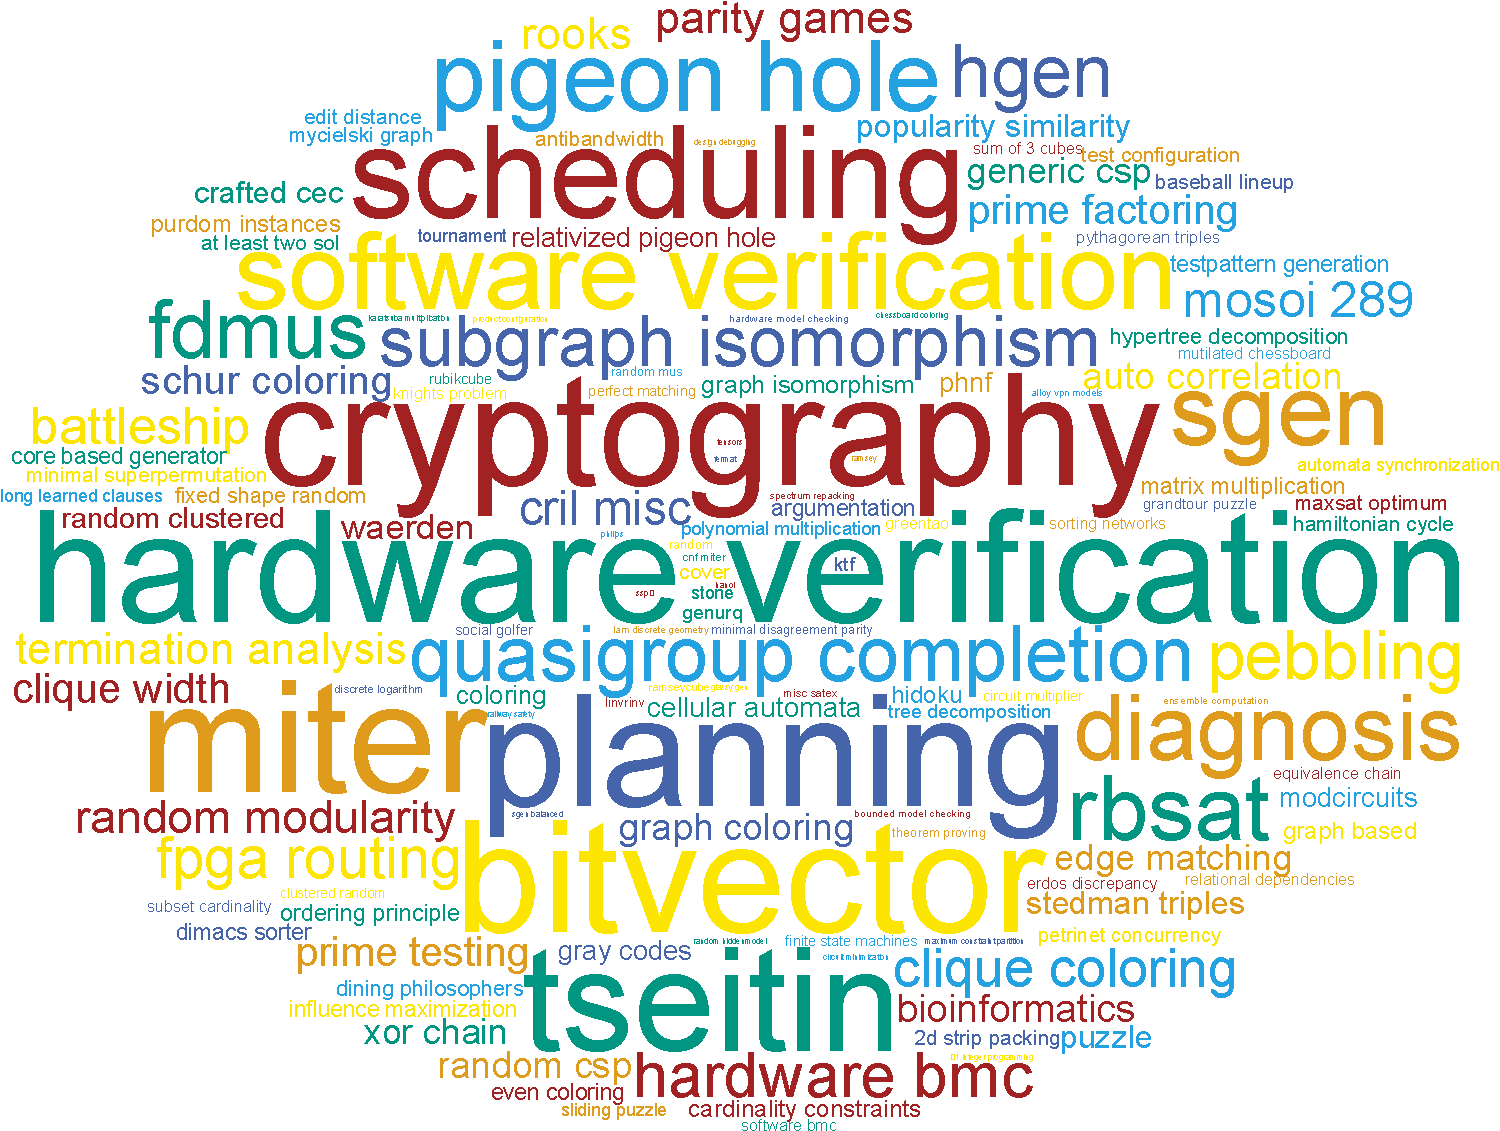
\includegraphics[height=6.5cm]{figures/l11/wordcloud3-crop.pdf}
	\end{minipage}%
	\begin{minipage}{0.27\textwidth}
		\centering
		{
			\small{}
			5355 problems,\\
			138 families + 72 unknown\\[3mm]
			Font size\ \,$\propto$\ \,\#\,problems\\[3mm]
			via \url{wordclouds.com},\\
			GBD (\url{benchmark-database.de})
		}
	\end{minipage}%
\end{frame}

\begin{frame}{Overview}
	\textbf{Selected (!) Application Highlights of SAT}
	\begin{itemize}
		\item \textcolor{gray}{Recap: Planning}
		\item Bounded Model Checking
		\item Combinational Equivalence Checking
		\item Analyzing Cryptographic Building Blocks
		\item Multi Agent Path Finding
		\item Explainable AI: Learning decision trees
		\item Train scheduling with disruptions via MaxSAT
	\end{itemize}
	\begin{block}{Remark}
		This slide set contains \highl{many literature references}---please follow them according to your interest!
	\end{block}
\end{frame}

\begin{frame}{Recap: Planning}
	\begin{itemize}
		\item \textbf{World state} $s$: Set of Boolean features
		\begin{itemize}
			\item Assert \highl{initial state} $s_I$ via unit clauses for \highl{time step 0}
			\item Assert \highl{goal state features} $g$ via unit clauses for \highl{time step $k$}
		\end{itemize}
		\item \textbf{Action}: Template for valid \highl{state transitions} $s_x \rightsquigarrow s_{x+1}$
		\begin{itemize}
			\item Executing an action at step $k$ implies its \highl{preconditions} at step $k$
			\item Executing an action at step $k$ implies its \highl{effects} at step $k+1$
		\end{itemize}
		\item \textbf{Plan}: Valid sequence of actions leading from $s_I$ to a goal state
		\begin{itemize}
			\item Sequence of action variables \highl{set to true} in satisfying assignment
		\end{itemize}
		\item Anything else to encode? \uncover<2->{\highlo{Frame axioms -- don't let the solver hallucinate causeless state changes!}}
	\end{itemize}
	\vspace*{5mm}
	\centering
	
\includegraphics[width=0.6\textwidth]{figures/l11/transition-system.pdf}
\end{frame}

% https://link.springer.com/content/pdf/10.1023/A:1011276507260.pdf
\begin{frame}{From Planning to Verification}
	\begin{minipage}[c][8cm][t]{0.65\textwidth}
		Let's use our SAT-based planning to \highl{check the correctness of a system}!
		\begin{itemize}
			\item World state features $\equiv$ State features of our system
			\item Actions $\equiv$ Valid \highl{transitions between states}
			\item Goals $\equiv$ \uncover<2->{\highl{incorrect state, violating some constraint}}
			\item<2-> Plan $\equiv$ \uncover<3->{\highlo{reachable incorrectness}}
			\item<3-> \highlo{Unsatisfiability}\only<4->{ \highlo{at $k$ steps}} $\equiv$ \only<3>{\highl{system is always correct?}}%
			\only<4->{\highl{system is correct \highlo{within $k$ steps}}}
		\end{itemize}
		\vspace*{3mm}
		\uncover<5->{
		\begin{block}{\textbf{Bounded Model Checking}}
			\begin{itemize}
				\item Encode and check \highl{transition system} for $k=1,2,\ldots$
				\item Satisfying assignment $\equiv$ \highlo{counter example}!
				\item Crucial tool for \highl{hardware and software verification}~\cite{vizel2015boolean}
			\end{itemize}
		\end{block}
		}
	\end{minipage}%
	\begin{minipage}[c][8cm][t]{0.35\textwidth}
		\centering
		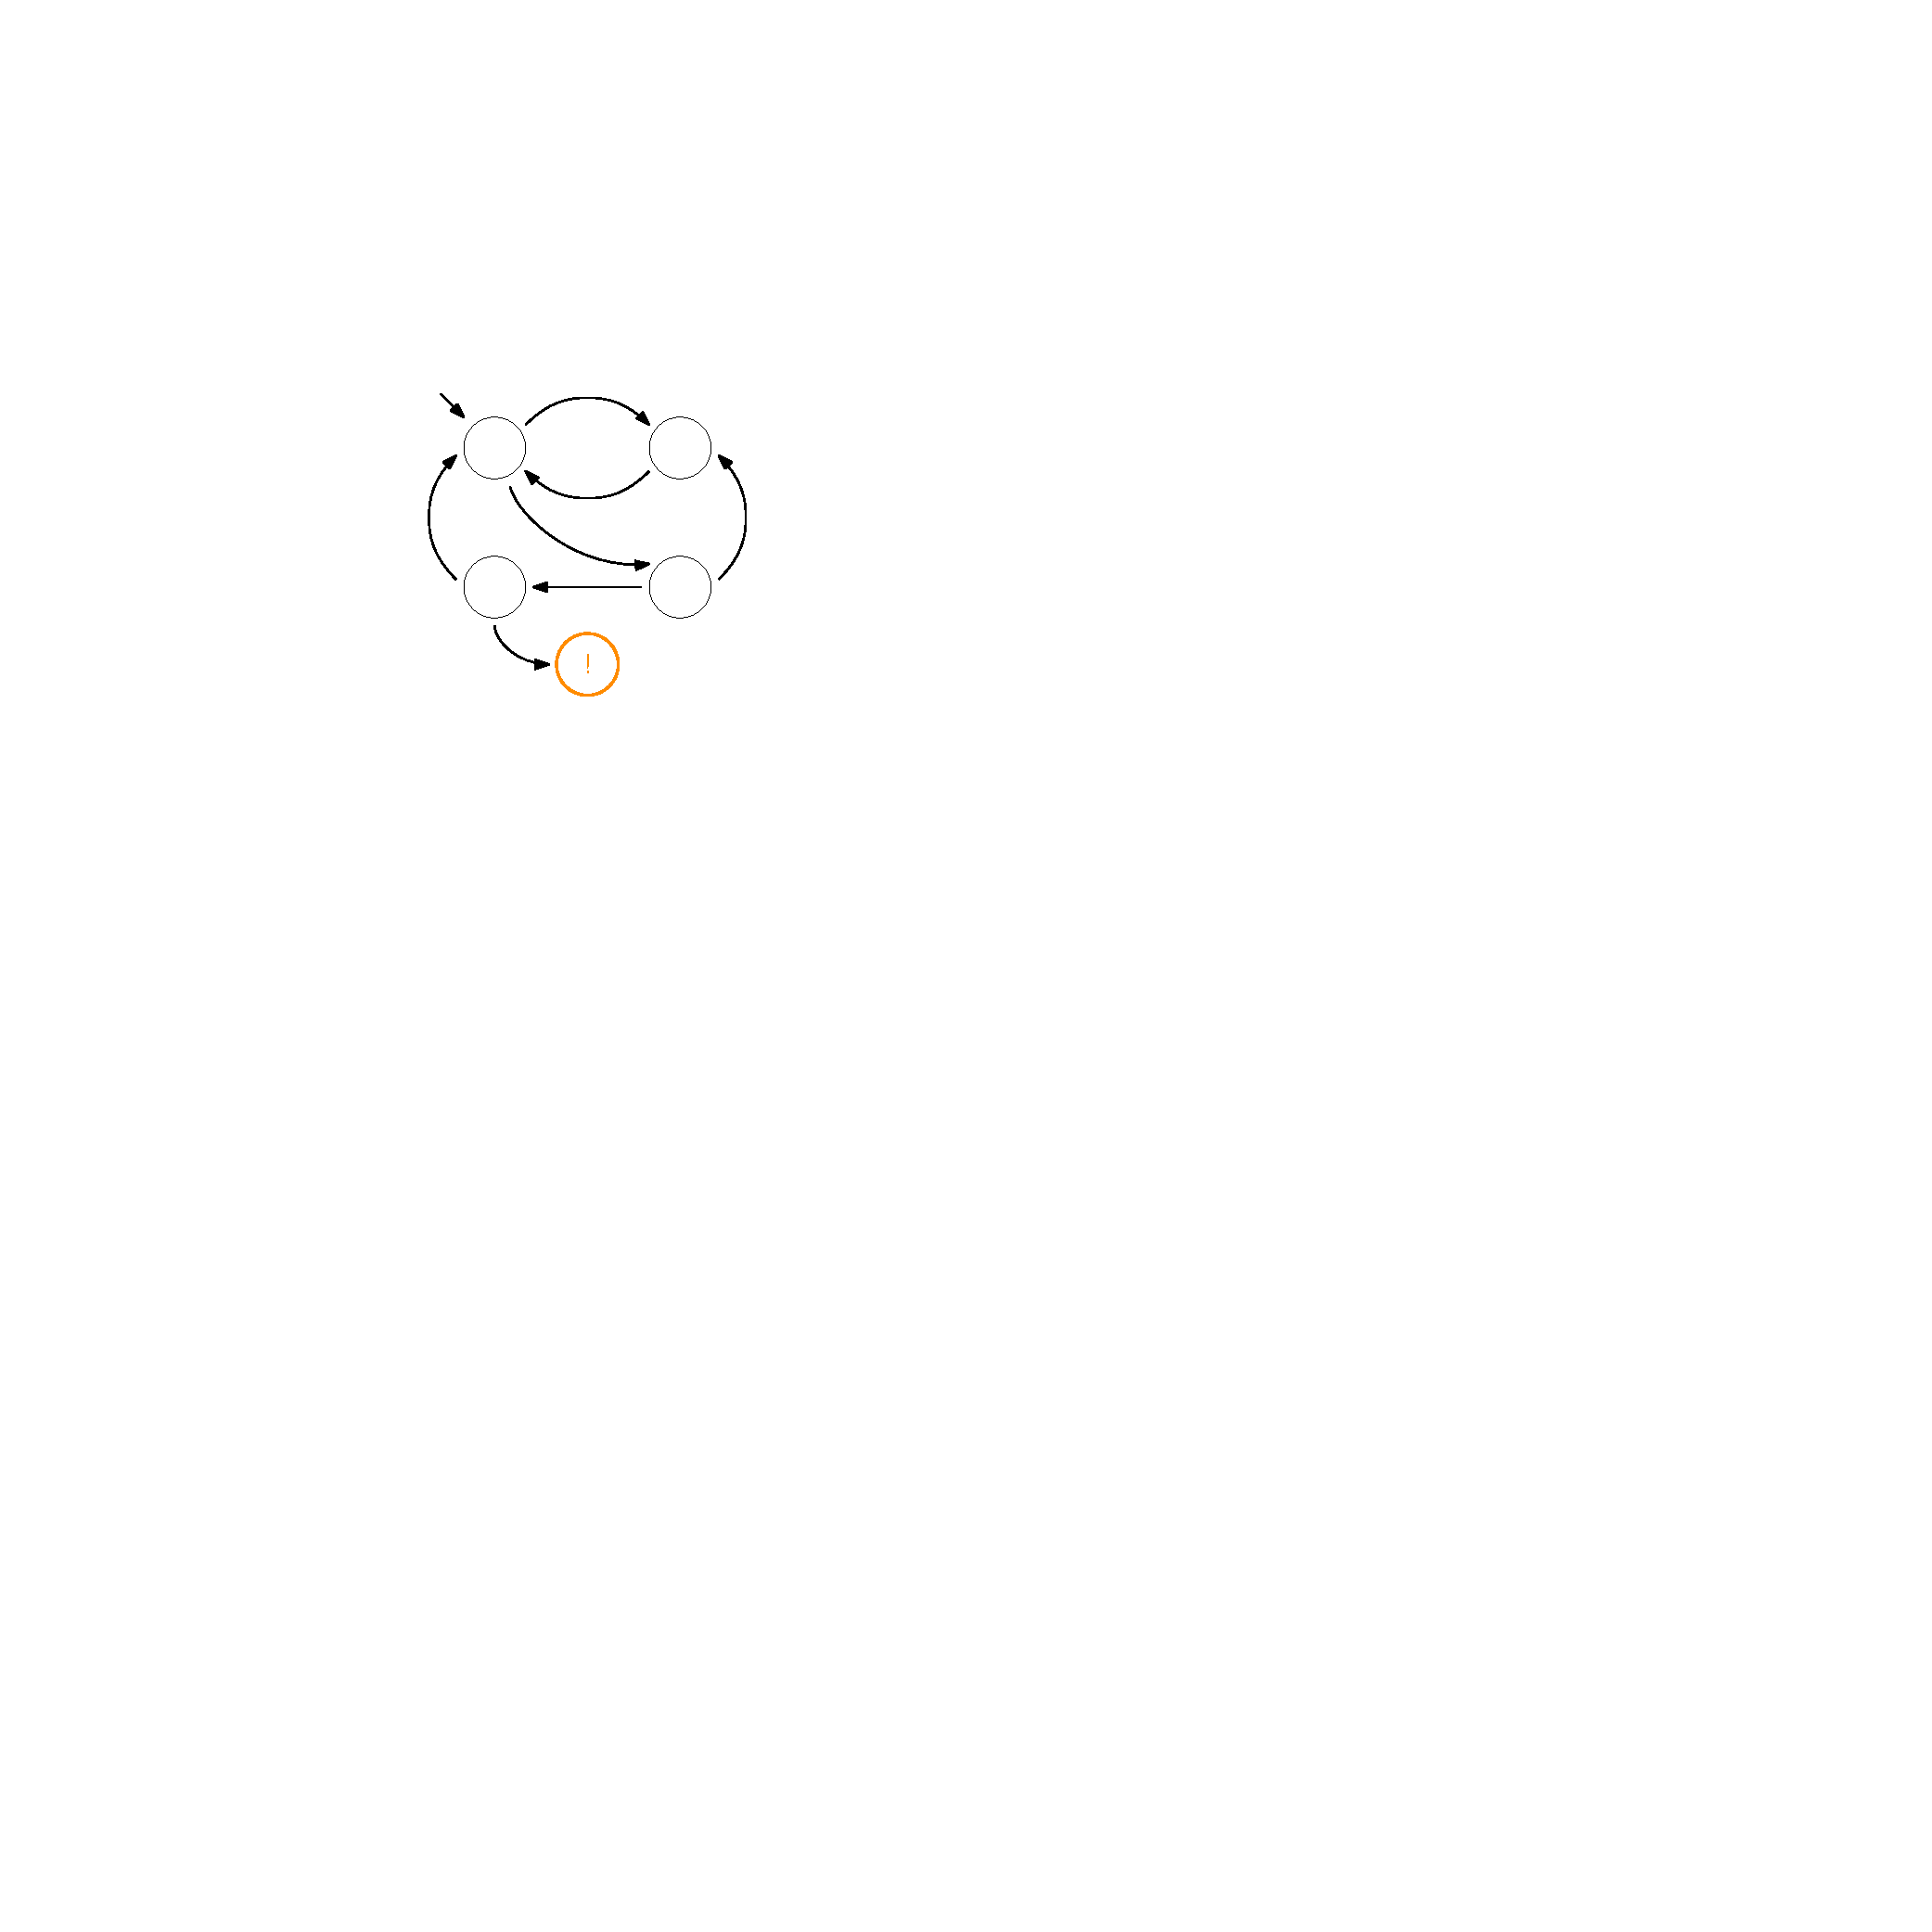
\includegraphics[width=0.9\textwidth]{figures/l11/transition-system-bmc.pdf}\\
		\textcolor{gray}{A snack machine or an electronic component or a C program or \ldots}
	\end{minipage}%
\end{frame}

\begin{frame}{Bounded Model Checking}
	\begin{minipage}[c][8cm][t]{0.6\textwidth}
		\begin{itemize}
			\item Invented by Clarke \& Biere in $\sim$2000~\cite{clarke2001bounded}, mostly replacing \highlo{BDD-based model checking}
			\item Uses state transition system based on \highl{temporal logic}\\(LTL, CTL, \ldots)
			\item Applications: Computer-aided design (CAD), software verification, invariant checking, bug detection, \ldots~\cite{vizel2015boolean}
			\item<2-> One of the \highl{most essential real-world applications} of SAT
			\begin{itemize}
				\item Pushed industrial interest in SAT solvers in 2000s
				\item Actively influenced solver design and algorithms
				\item Some of the \highl{largest, structurally most distinct} benchmarks
			\end{itemize}
			\item<3-> Examples for BMC @ KIT:
			\begin{itemize}
				\item \highl{Low-Level Bounded Model Checker} (LLBMC)~\cite{falke2013bounded}\\(C program verification)
				\item Verification of Java contracts~\cite{beckert2020modular} \unimp{(see right)}
				\item Cryptography~\cite{koch2021card}
			\end{itemize}
		\end{itemize}
	\end{minipage}%
	\begin{minipage}[c][8cm][t]{0.4\textwidth}
		\centering
		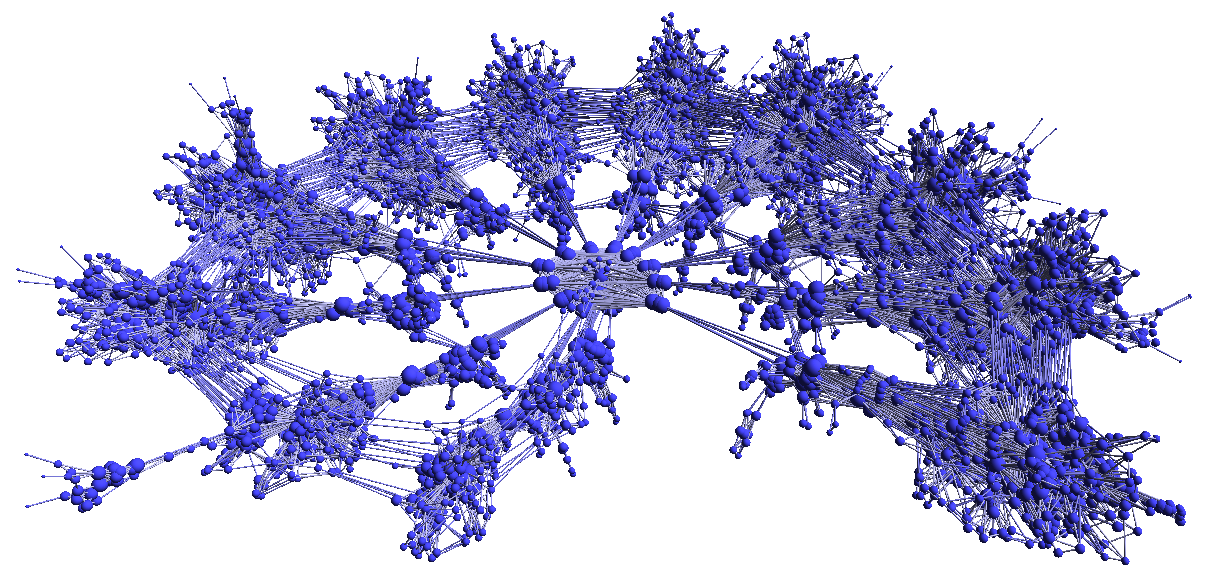
\includegraphics[width=0.9\textwidth]{figures/l11/bmc.png}
		%\\\textcolor{gray}{A Bounded Model Checking instance}
		\\[3mm]
		\uncover<3->{
		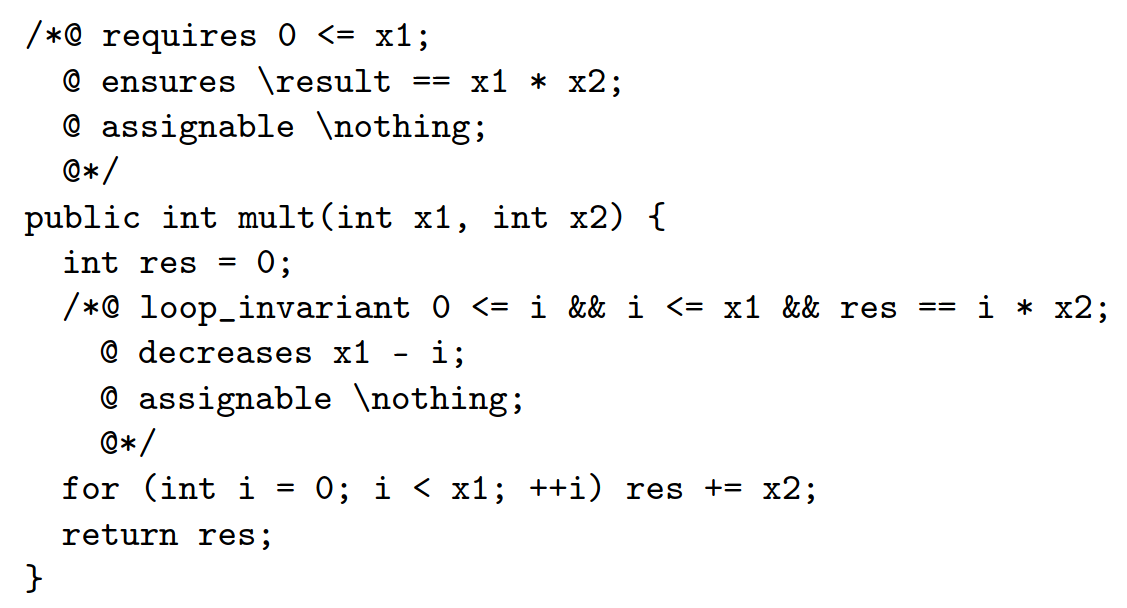
\includegraphics[width=\textwidth]{figures/l11/jml.png}
		}
	\end{minipage}%
\end{frame}

\begin{frame}{Combinational Equivalence Checking}
	% https://www21.in.tum.de/~lammich/2015_SS_Seminar_SAT/resources/Equivalence_Checking_11_30_08.pdf
	% https://ieeexplore.ieee.org/stamp/stamp.jsp?tp=&arnumber=4196156
	\begin{minipage}[c][8cm][t]{0.5\textwidth}
		%\textbf{Example}: \highl{Combinational Equivalence Checking} (CEC)
		\begin{itemize}
			\item Given: two \highl{combinational circuits}\\
			\textcolor{gray}{stateless ``input$\rightarrow$output'' circuit, no feedback}
			\item Question: are the circuits \highl{logically equivalent}?
			\item {Right example: Is $F(a,b,c) \equiv G(a,b,c)$?}
			\item How to solve with SAT?
		\end{itemize}
	
		\vspace*{3mm}
		\uncover<2->{
		\begin{block}{Miter Formula}
			\begin{itemize}
				\item Encode $F$, $G$ relative to \highl{shared input bits}
				\item Assert $x \neq y$ (multi-bit output: $\bigvee_{x_i,y_i} x_i \neq y_i$)
				\item Satisfiable $\Leftrightarrow$ ($F \not\equiv G$)\hfill (\highlo{why this way?})\ \ 
			\end{itemize}
		\end{block}	
		}
	\end{minipage}%
	\begin{minipage}[c][8cm][t]{0.5\textwidth}
		\only<1>{
		\centering
		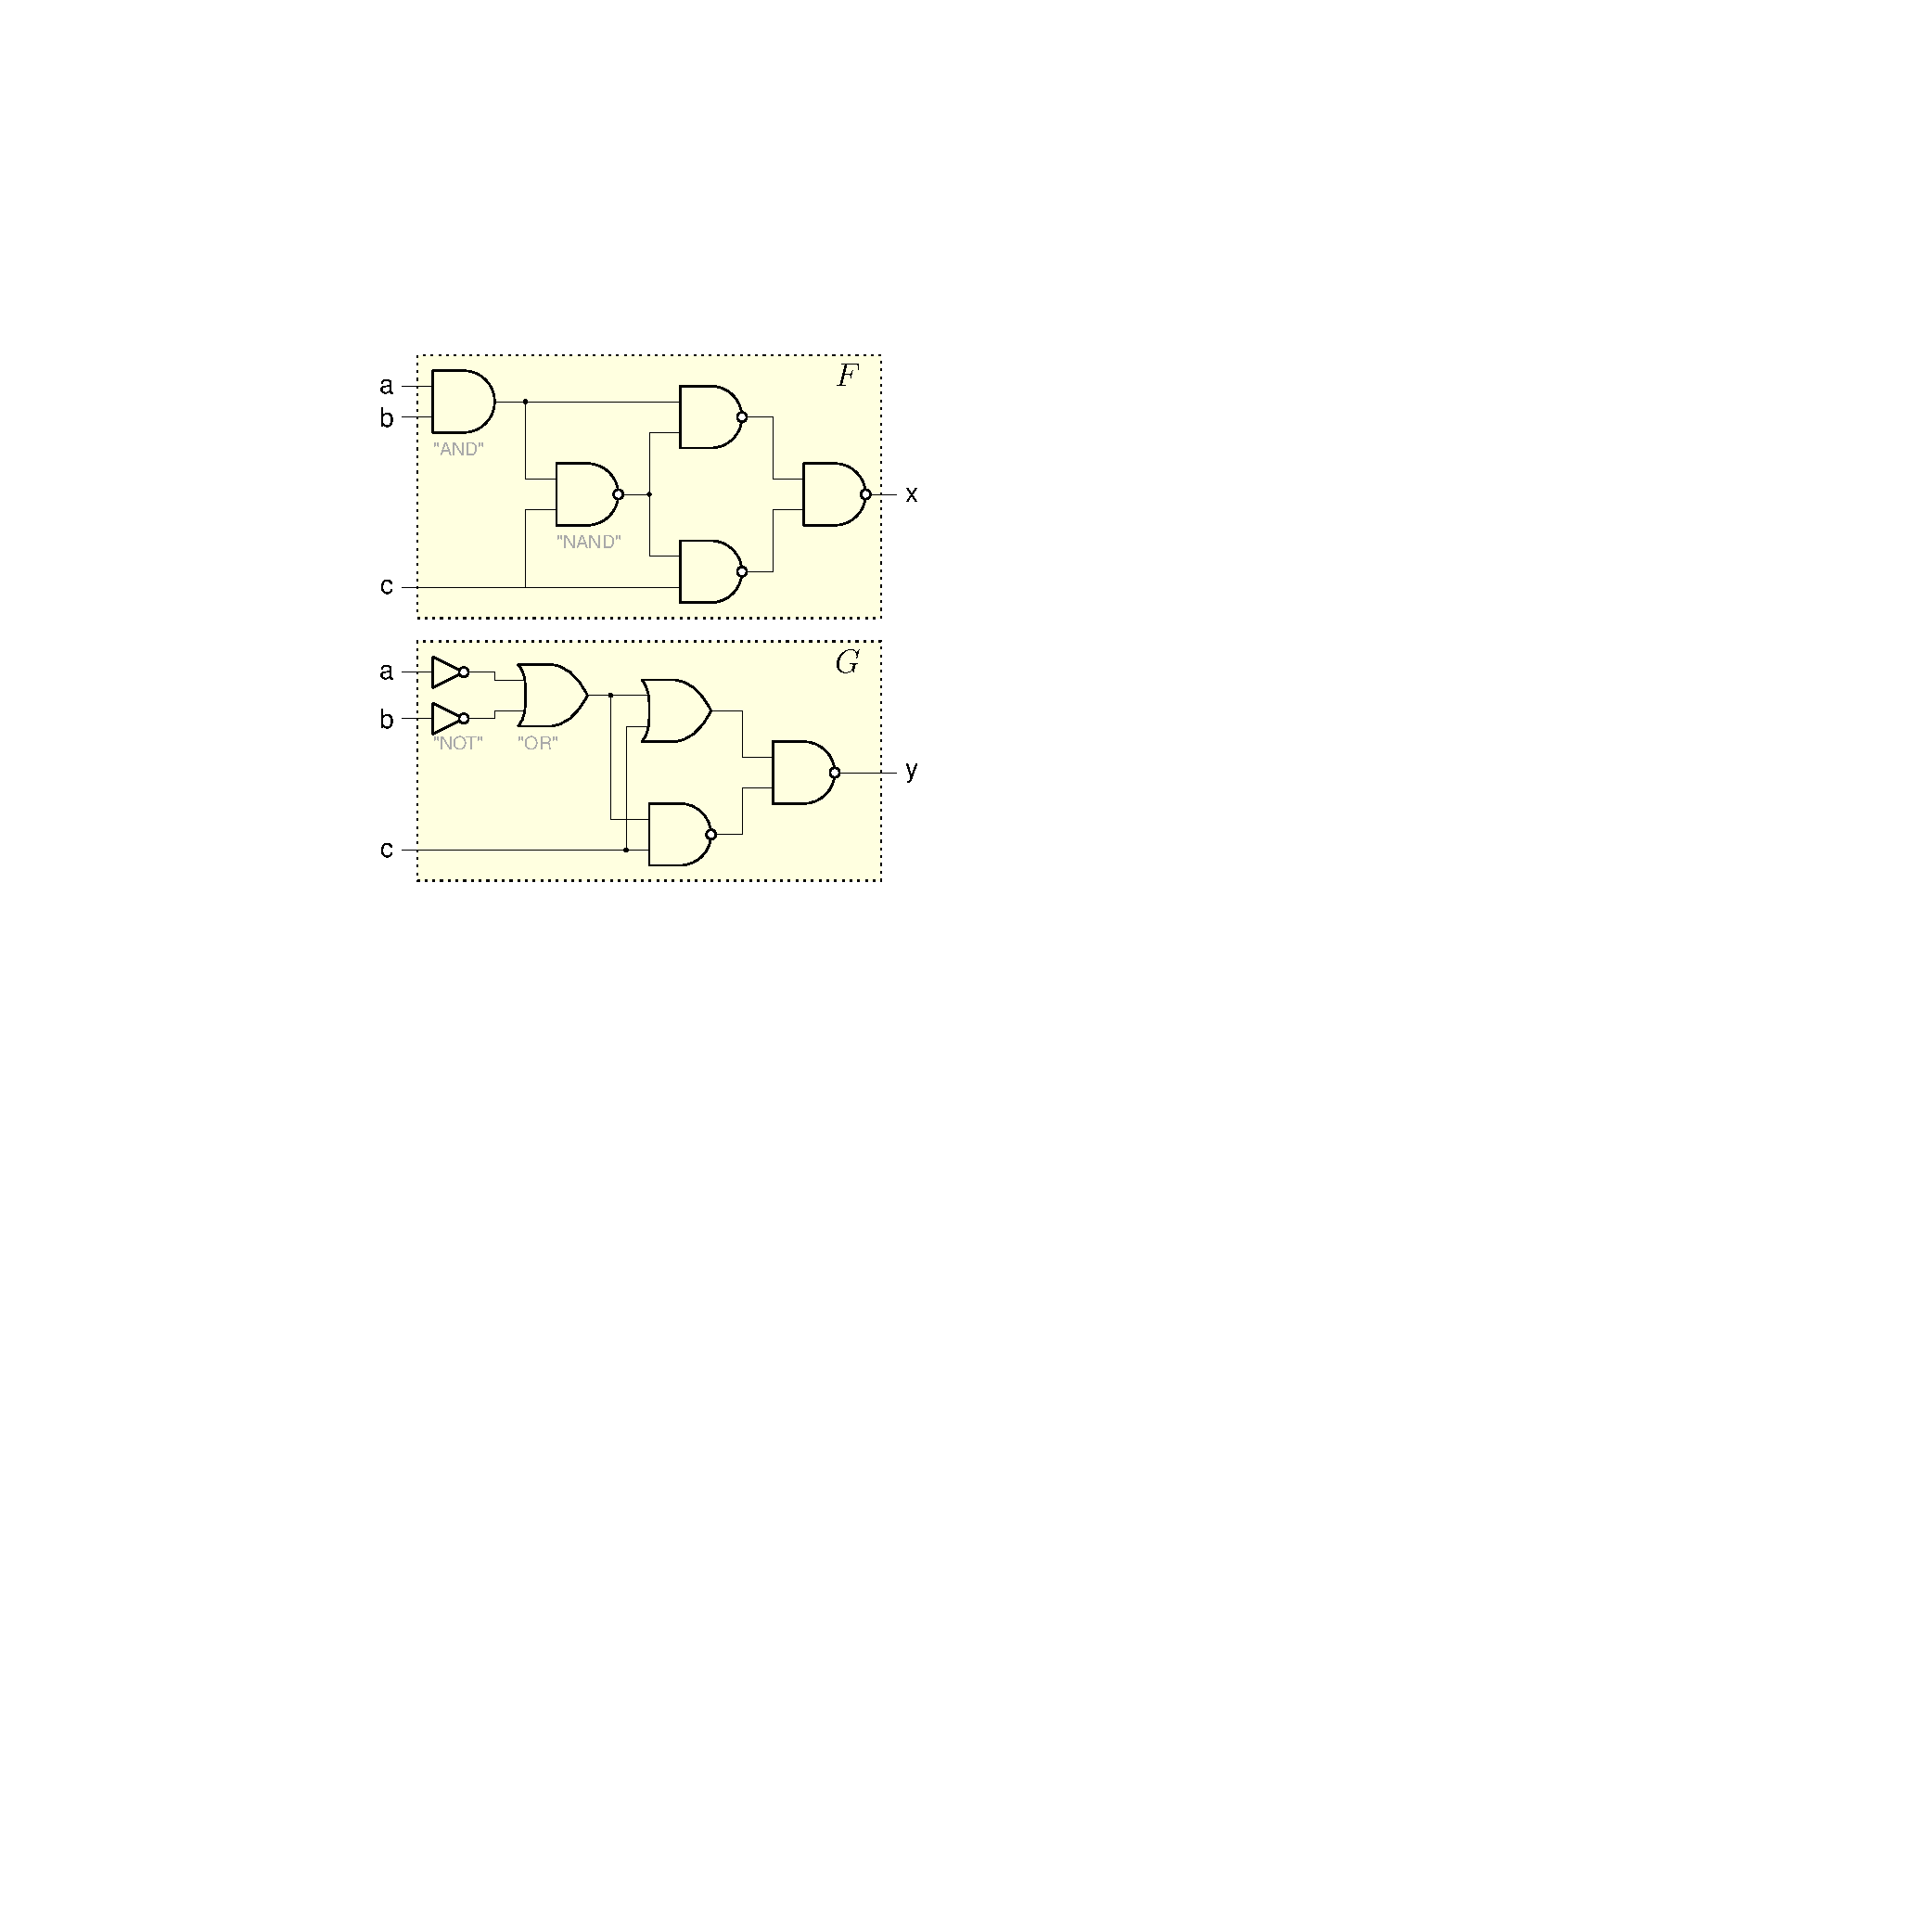
\includegraphics[width=0.8\textwidth]{figures/l11/circuits.pdf}
		}%
		\only<2->{
		\ \ 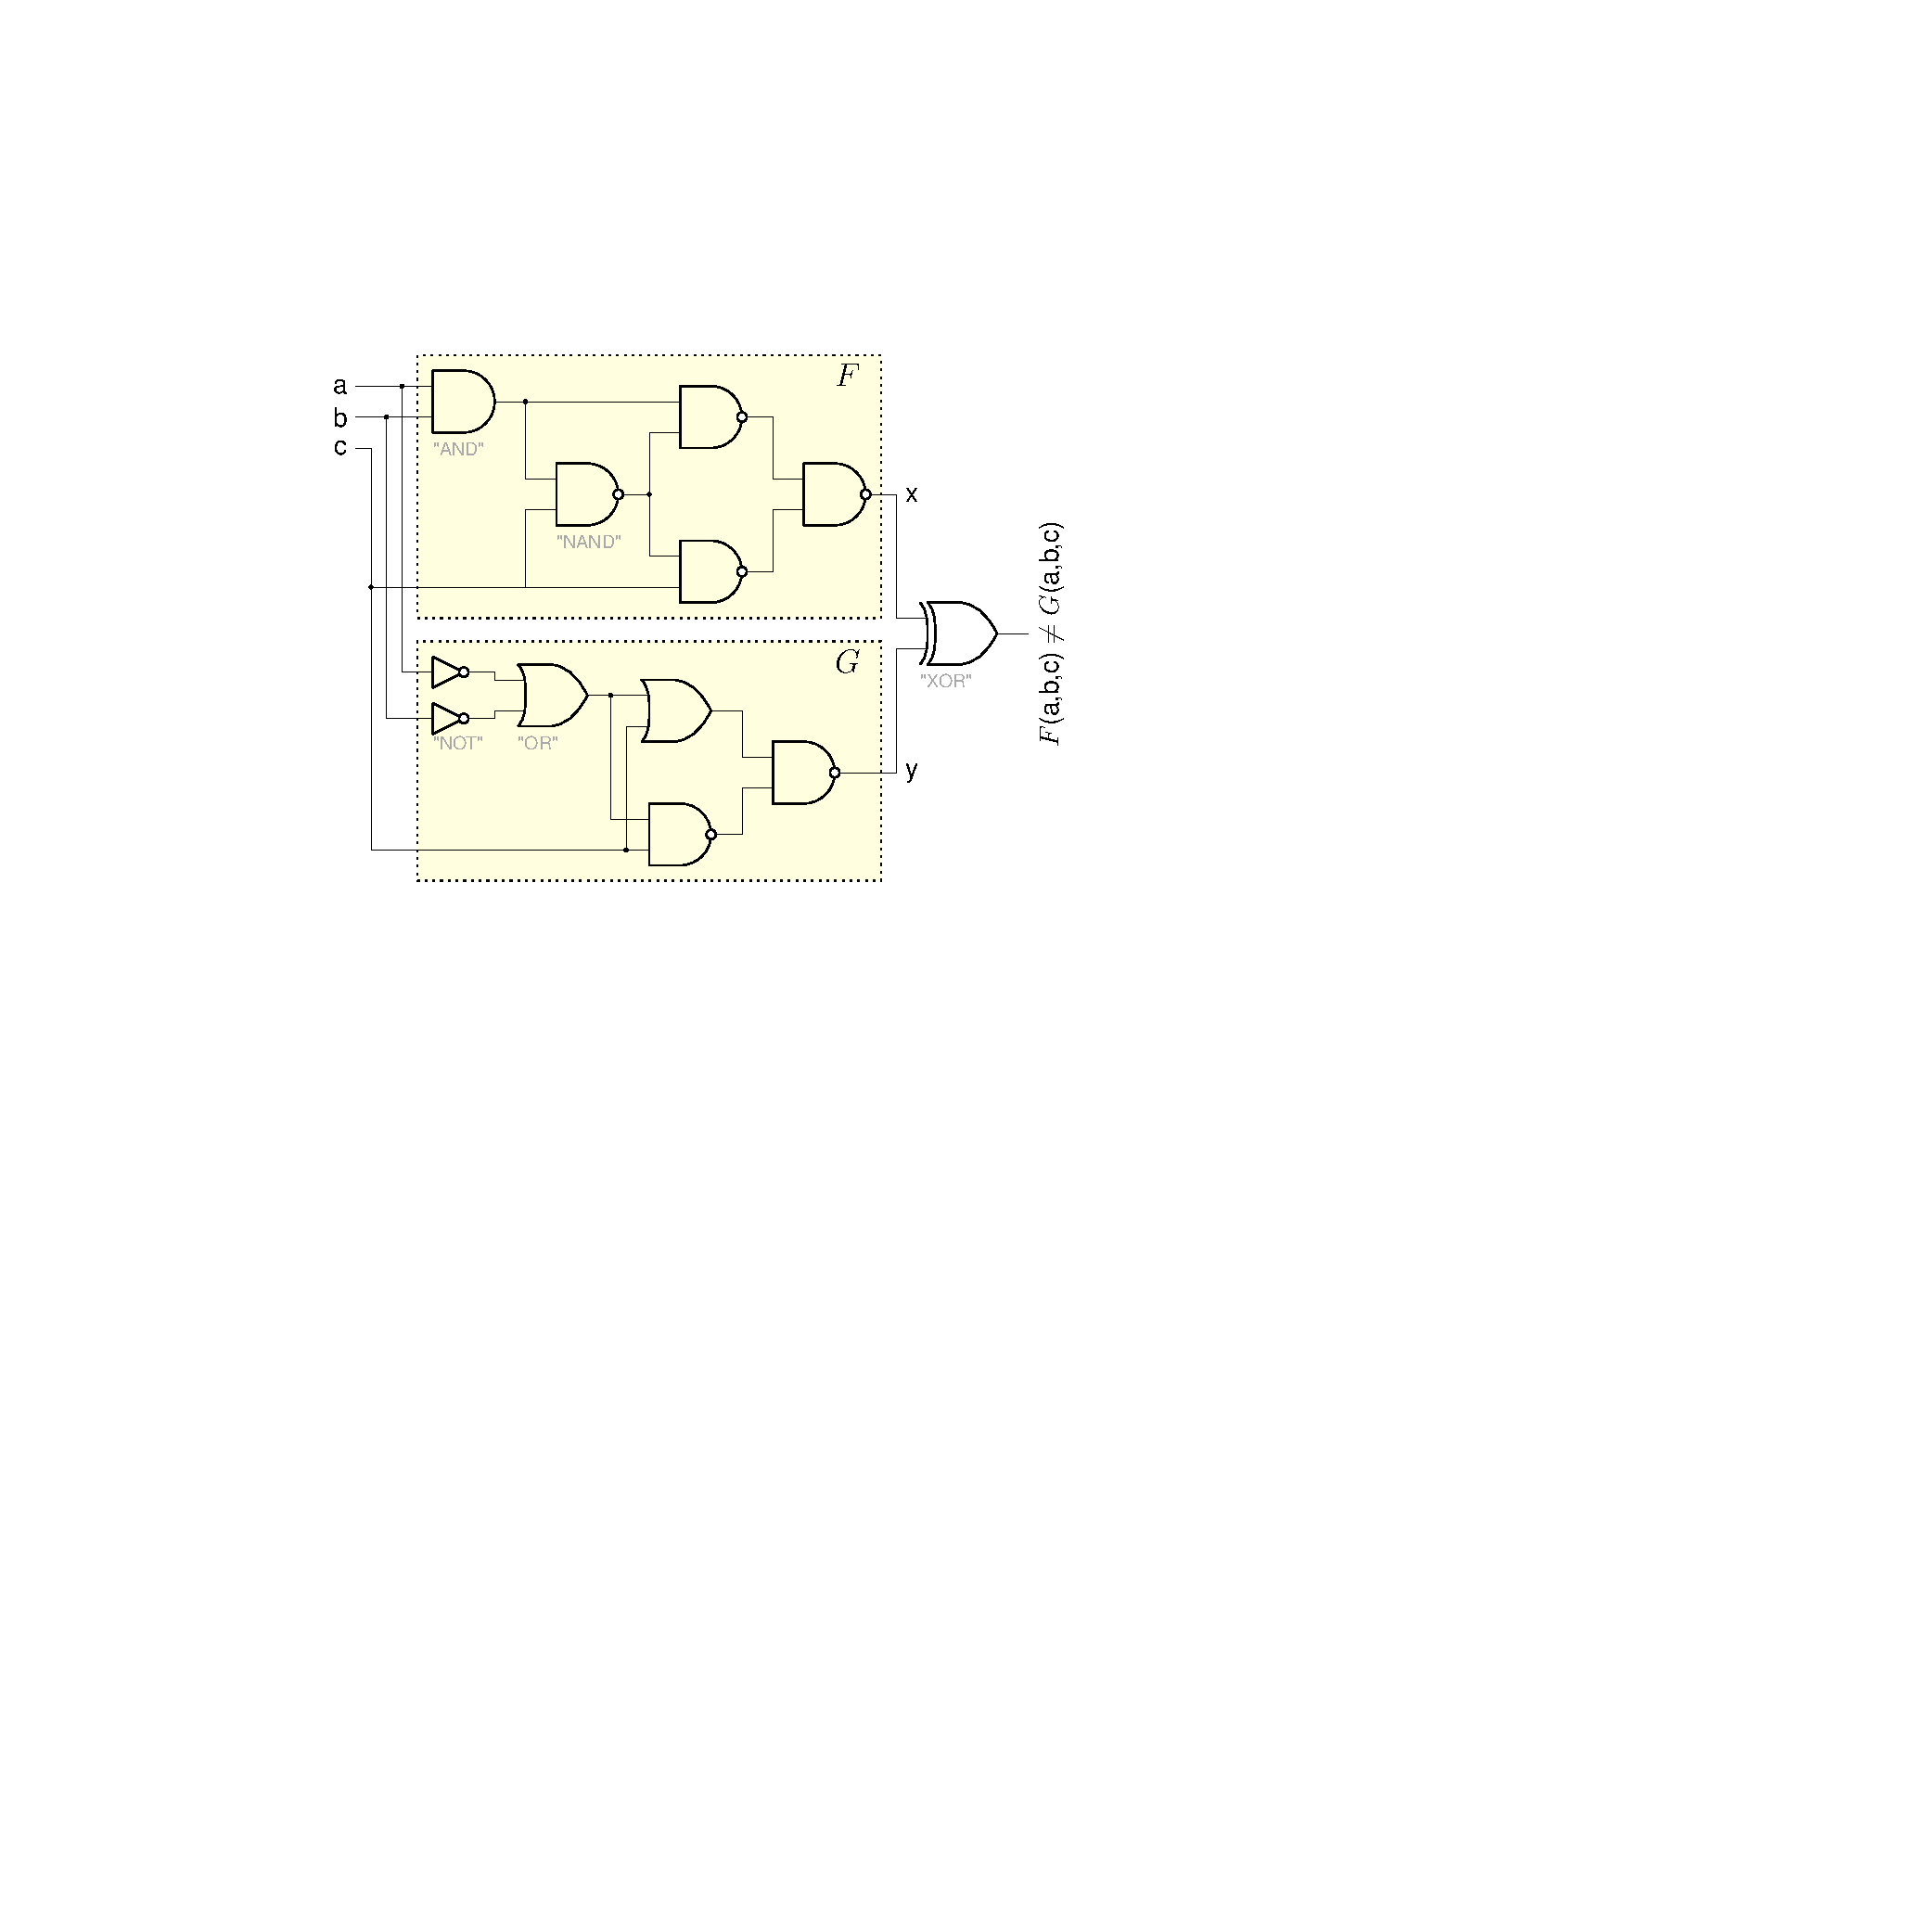
\includegraphics[width=\textwidth]{figures/l11/circuits-miter.pdf}
		}
	\end{minipage}%
\end{frame}

\begin{frame}{CEC: How Hard Can It Be?}
	\begin{minipage}[c][12cm][t]{0.57\textwidth}
		\vspace*{0.4cm}
		\textbf{Two Miter examples} from SAT Competition 2023%
		\begin{itemize}
			\vspace*{2mm}
			\uncover<1->{%
				\item Instance A:\ \ 260k variables, 850k clauses%
				\begin{itemize}
					\item Circuits are \highlo{not equivalent}
					%\\-- \highl{erfüllende Belegung} führt zu \highlo{unterschiedlichen Outputs}
					\item \highl{Solved in 1.33\,s} by \textsc{Kissat\_MAB\_prop-no\_sym}~\cite{gao2023kissat}
				\end{itemize}%
			}%
			\vspace*{1mm}%
			\uncover<2->{%
				\item Instance B:\ \ 4k variables, 13k clauses
				\begin{itemize}
					\item Circuits are \highl{equivalent} %--- alle Variablenbelegungen führen zu \highl{denselben Outputs}
					\item \highlo{Unsolved} by sequential solvers within 5000\,s
					\item Solved by some \highl{parallel solvers} :)
				\end{itemize}%
			}%
		\end{itemize}
		\vspace*{1mm}%
		\uncover<3->{%
		%	\begin{exampleblock}{Beobachtung}
		%		Es ergeben sich stets \highl{praktisch relevante} Probleme,\\
		%		die mit aktuellen Solvern \highlo{nicht praktikabel lösbar} sind.
		%	\end{exampleblock}
			\textbf{Generally:}	\highlo{co-NP-complete}, can require \highlo{very large proofs}	
		}	
	\end{minipage}%
	\begin{minipage}[c][12cm][t]{0.43\textwidth}
		\vspace*{0.5cm}
		\centering%
		\only<1>{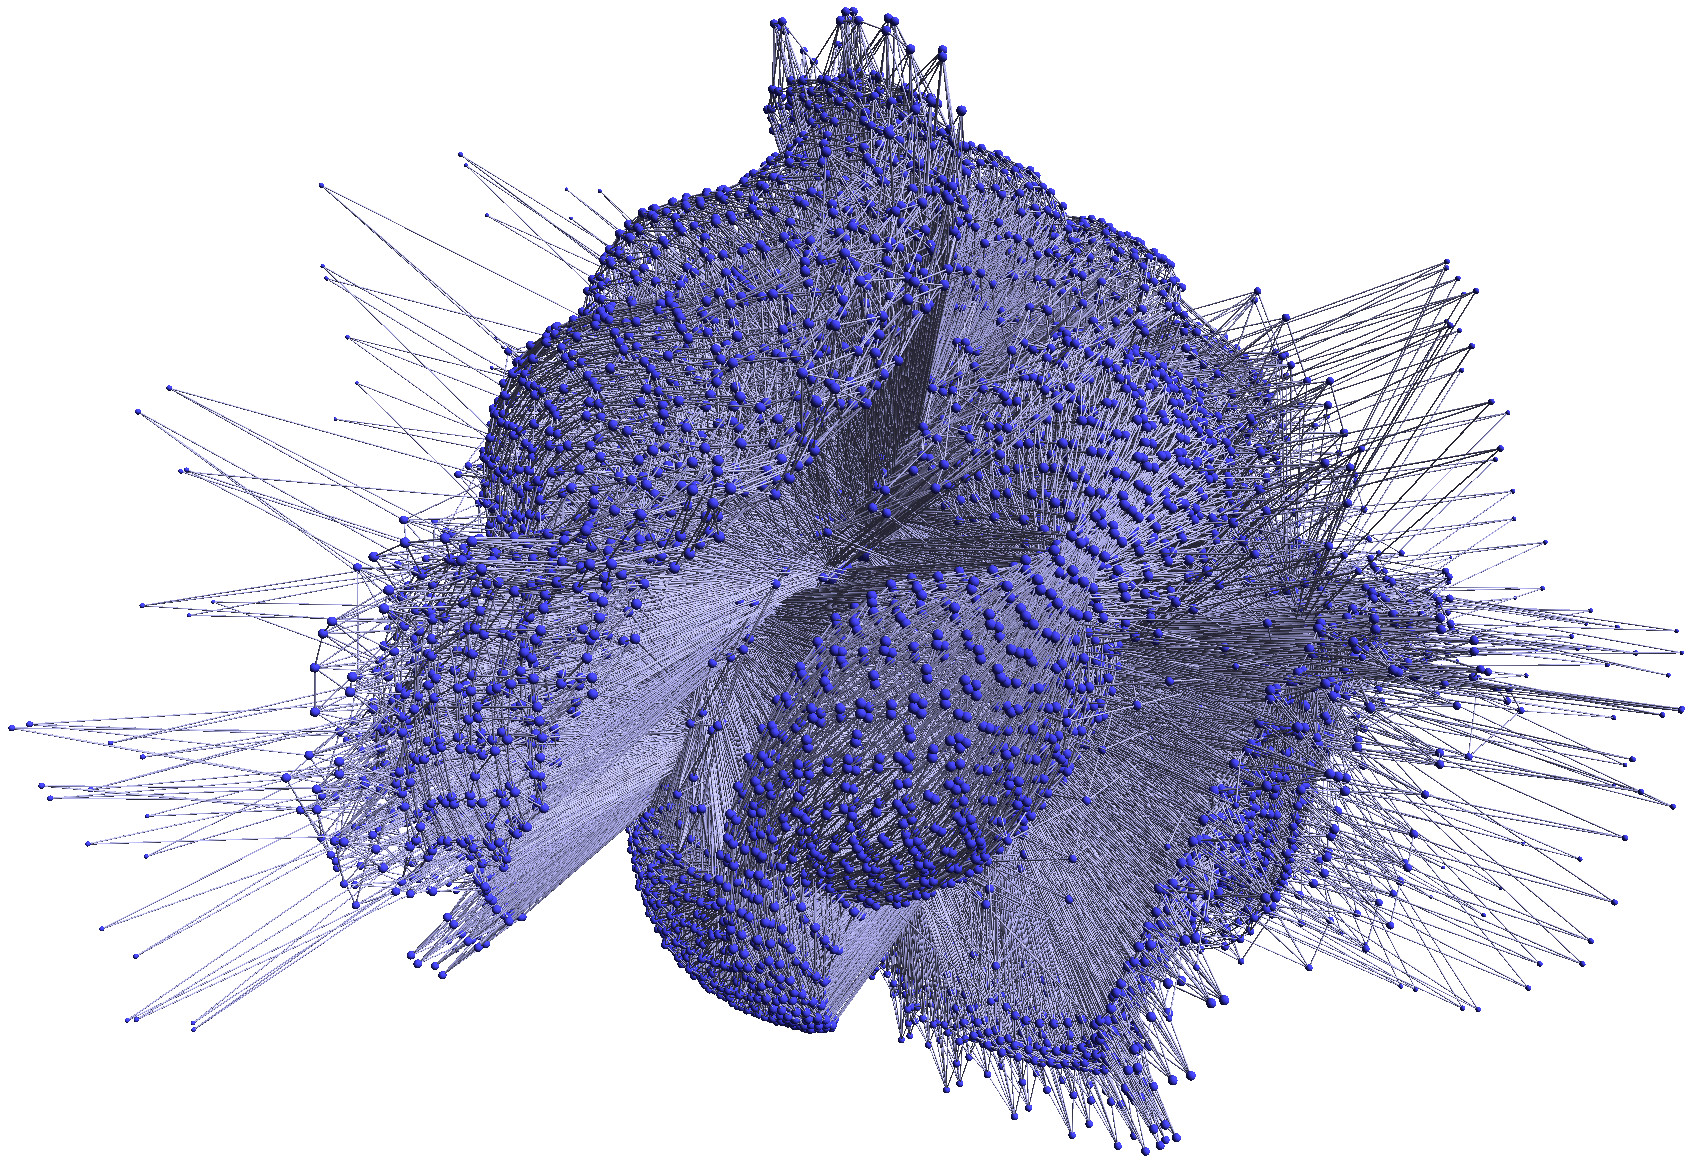
\includegraphics[width=0.95\textwidth]{figures/l11/3d-large-miter-visualization.jpg}%
			\\\unimp{\small Nodes = variables;\\Edges = common clause(s);\\
				variables contracted by factor $\approx$ 16}%
		}%
		\only<2->{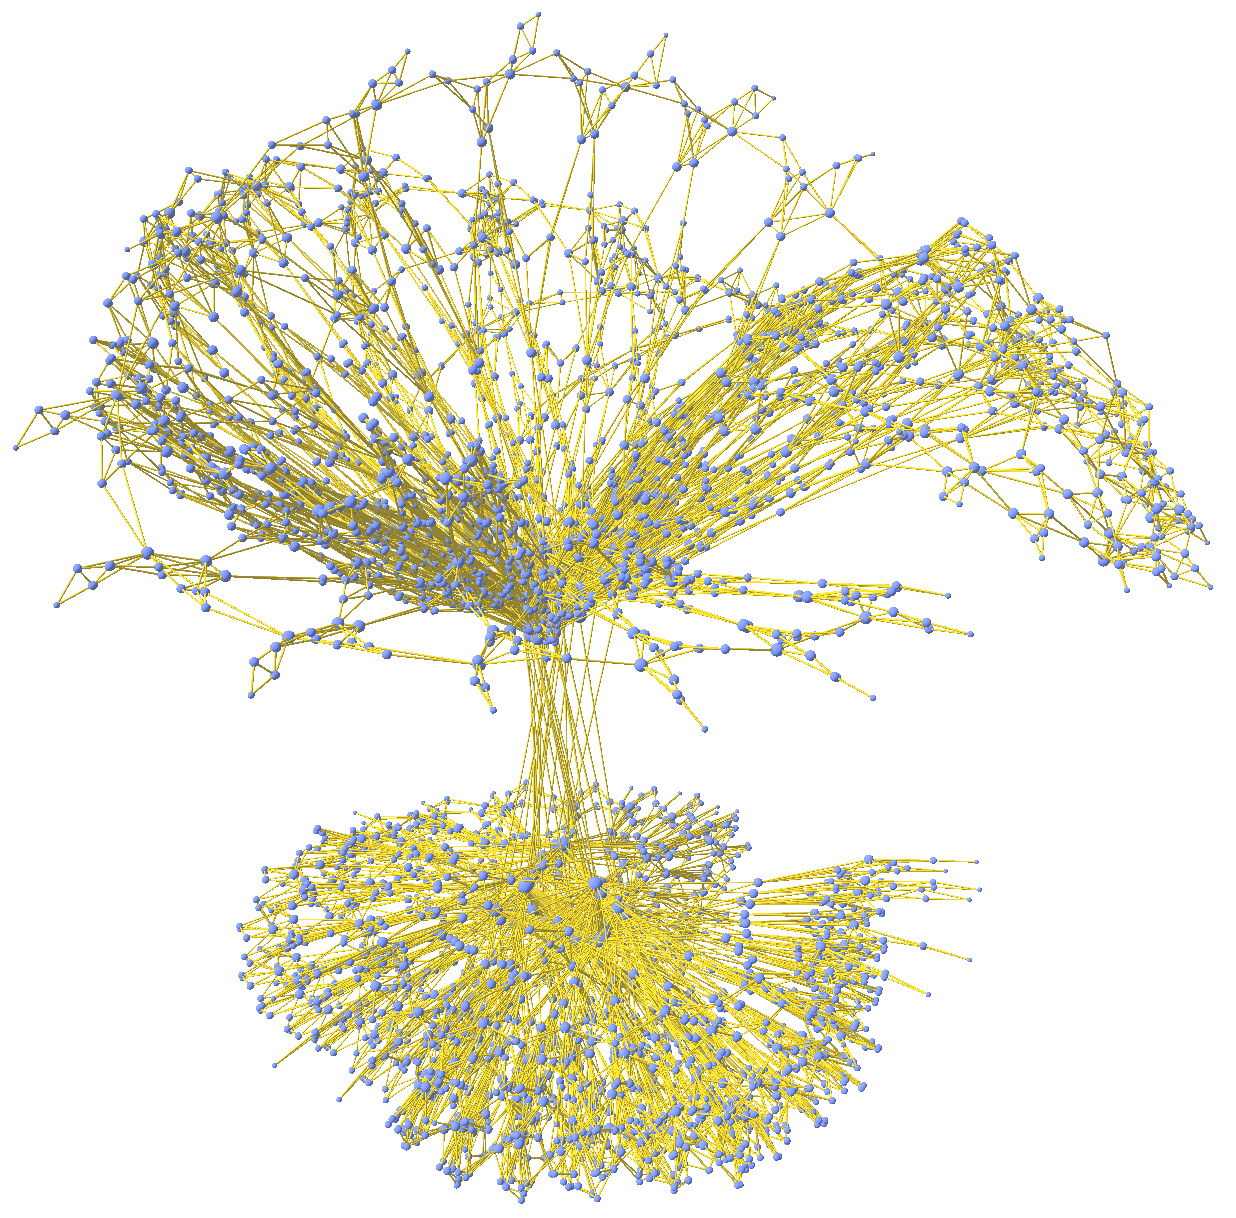
\includegraphics[width=0.7\textwidth]{figures/l11/3d-miter-visualization.jpg}%
			\\\unimp{\small Nodes = variables;\\Edges = common clause(s)}%
		}%
	\end{minipage}	
\end{frame}

\begin{frame}{CEC Techniques~\cite{weaver2015equivalence}}
	\begin{minipage}[c][8cm][t]{0.5\textwidth}
		\textbf{Improving CEC performance}: Try to \highl{merge equivalent sub-circuits}
		\begin{itemize}
			\item Randomly test different inputs, collecting pairs of \highl{potentially equivalent nodes}
			\item<2-> Use \highl{And/Inverter-Graph} (AIG) for simple circuit manipulation and merging
			\item<7-> \highl{Structural hashing}: Ensure that each functionally distinct sub-circuit is encoded \highl{only once}
			\item<8-> \highl{SAT sweeping}:
			Use \highl{SAT sub-program} to test whether potentially equivalent nodes are actually equivalent
		\end{itemize}
	\end{minipage}%
	\begin{minipage}[c][8cm][t]{0.5\textwidth}
		\centering%
		\only<1>{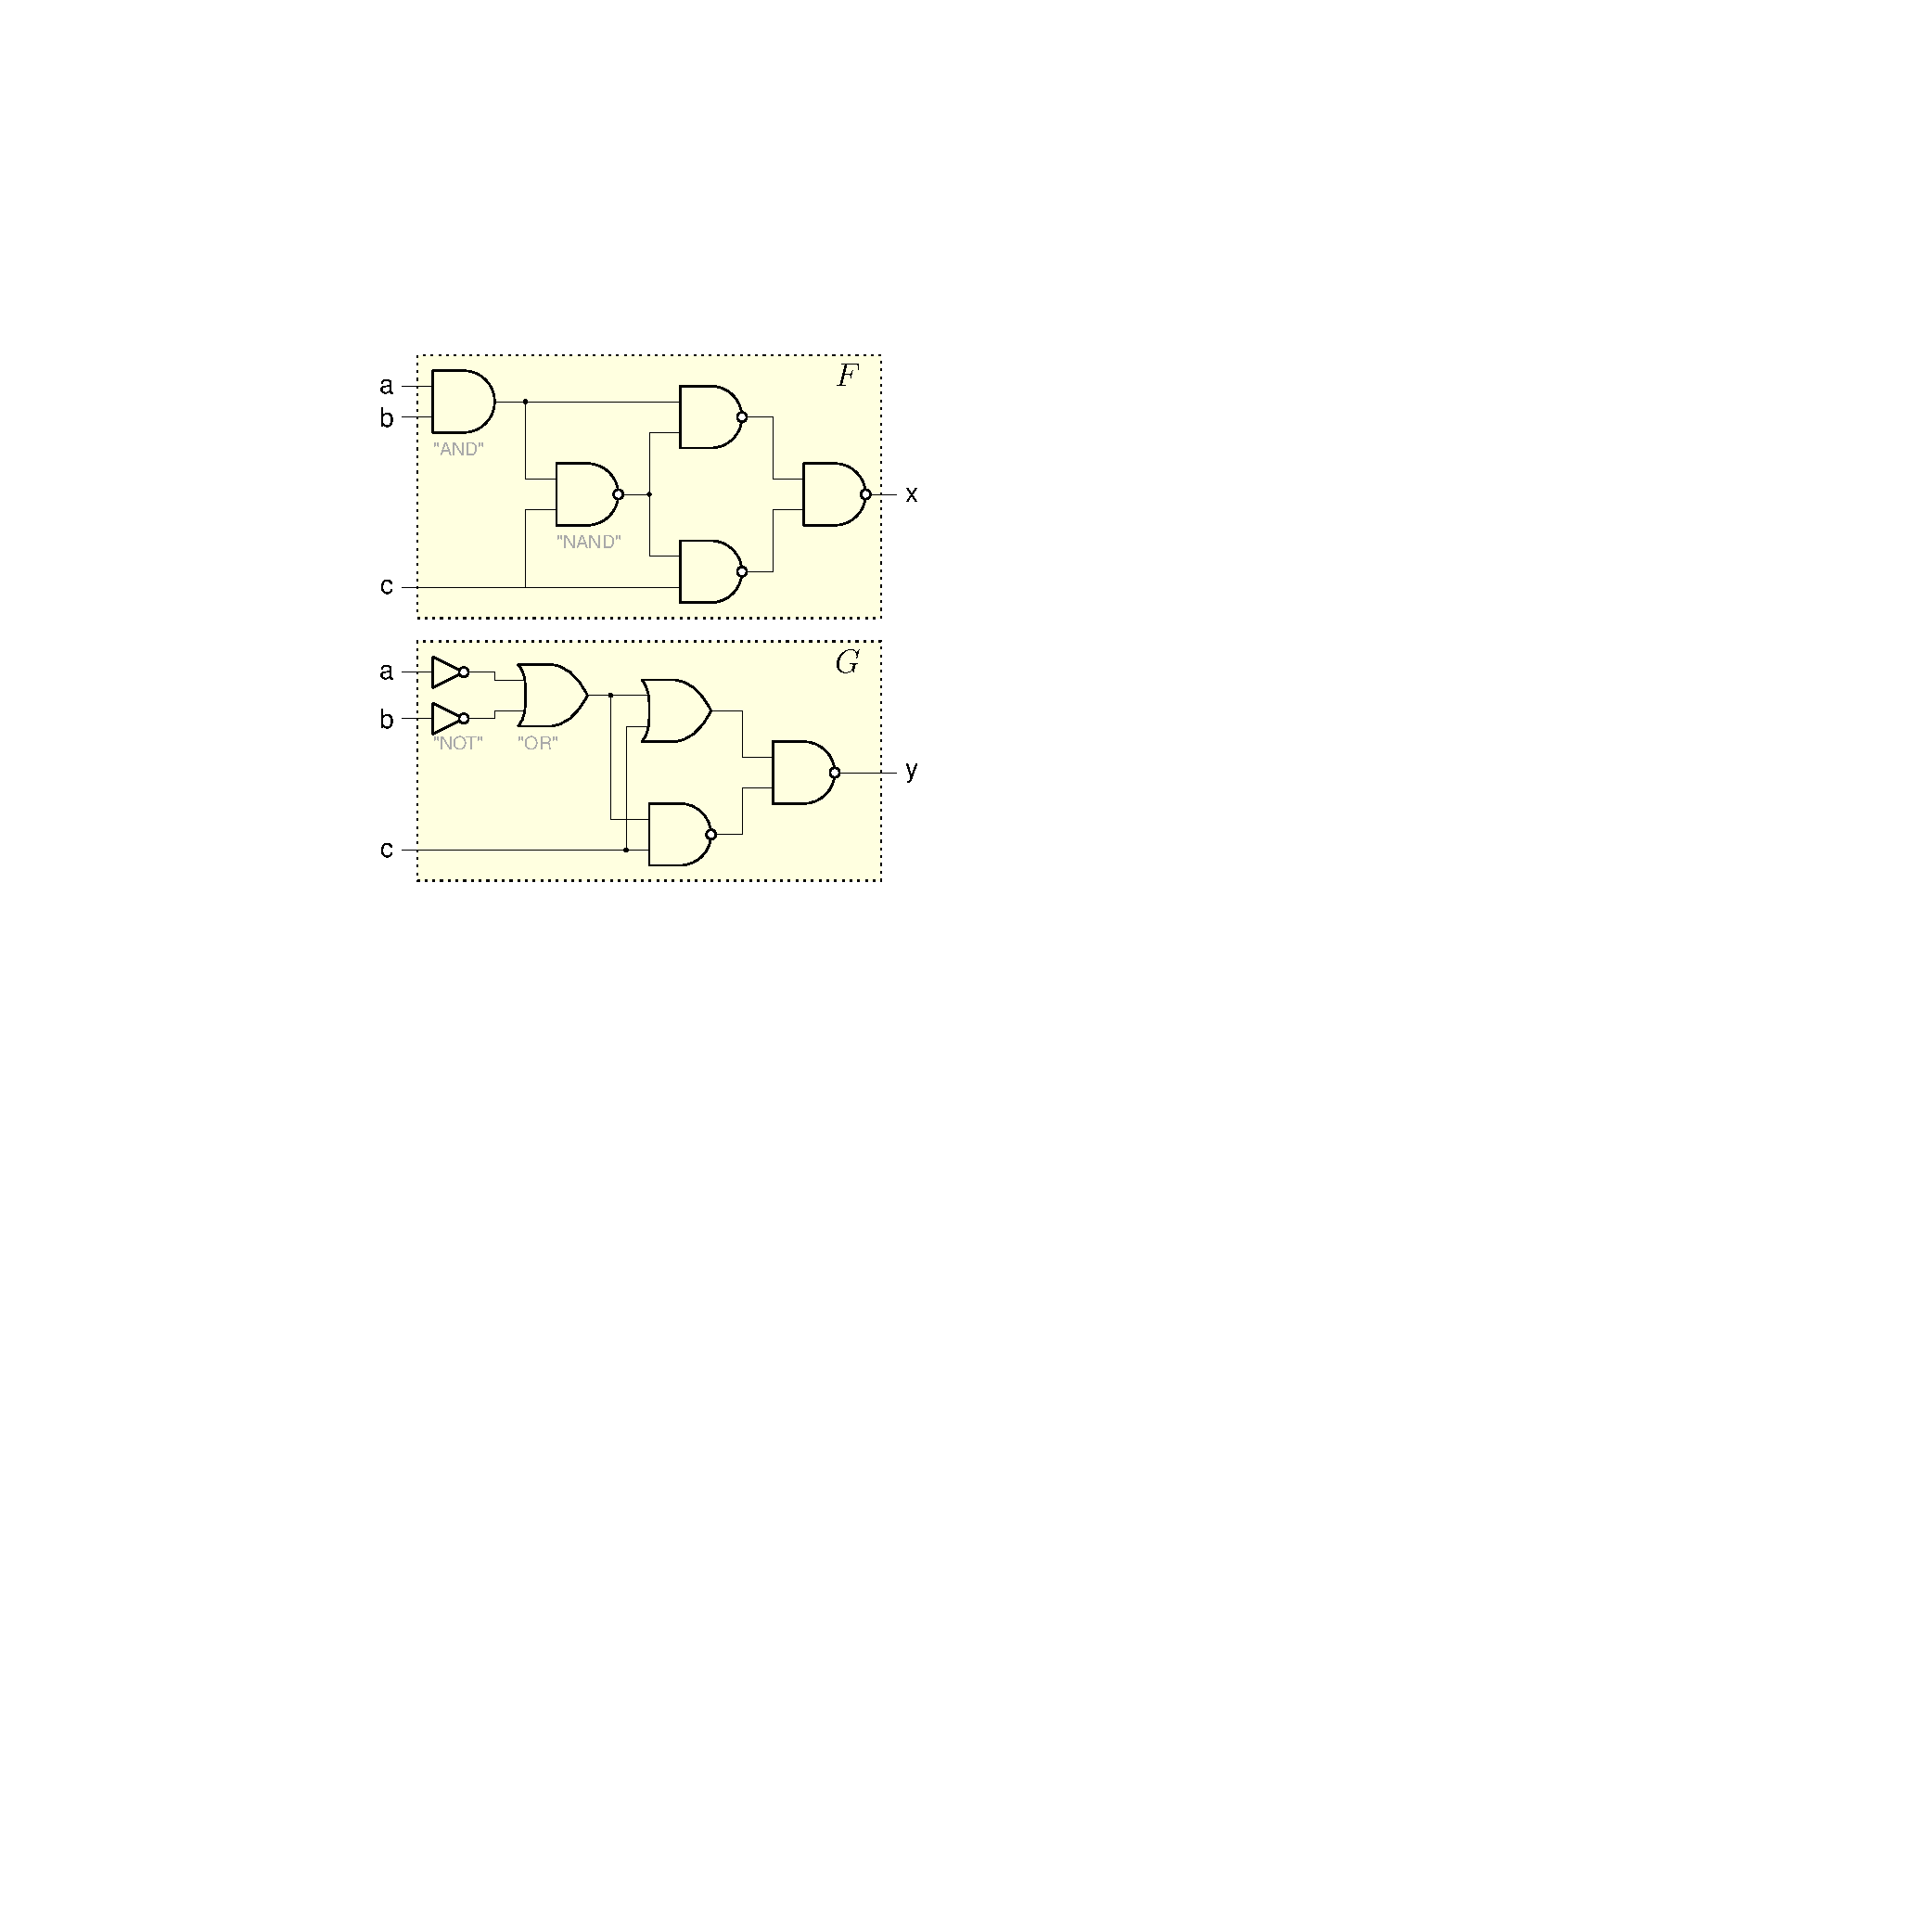
\includegraphics[width=0.8\textwidth]{figures/l11/circuits.pdf}}%
		\only<2>{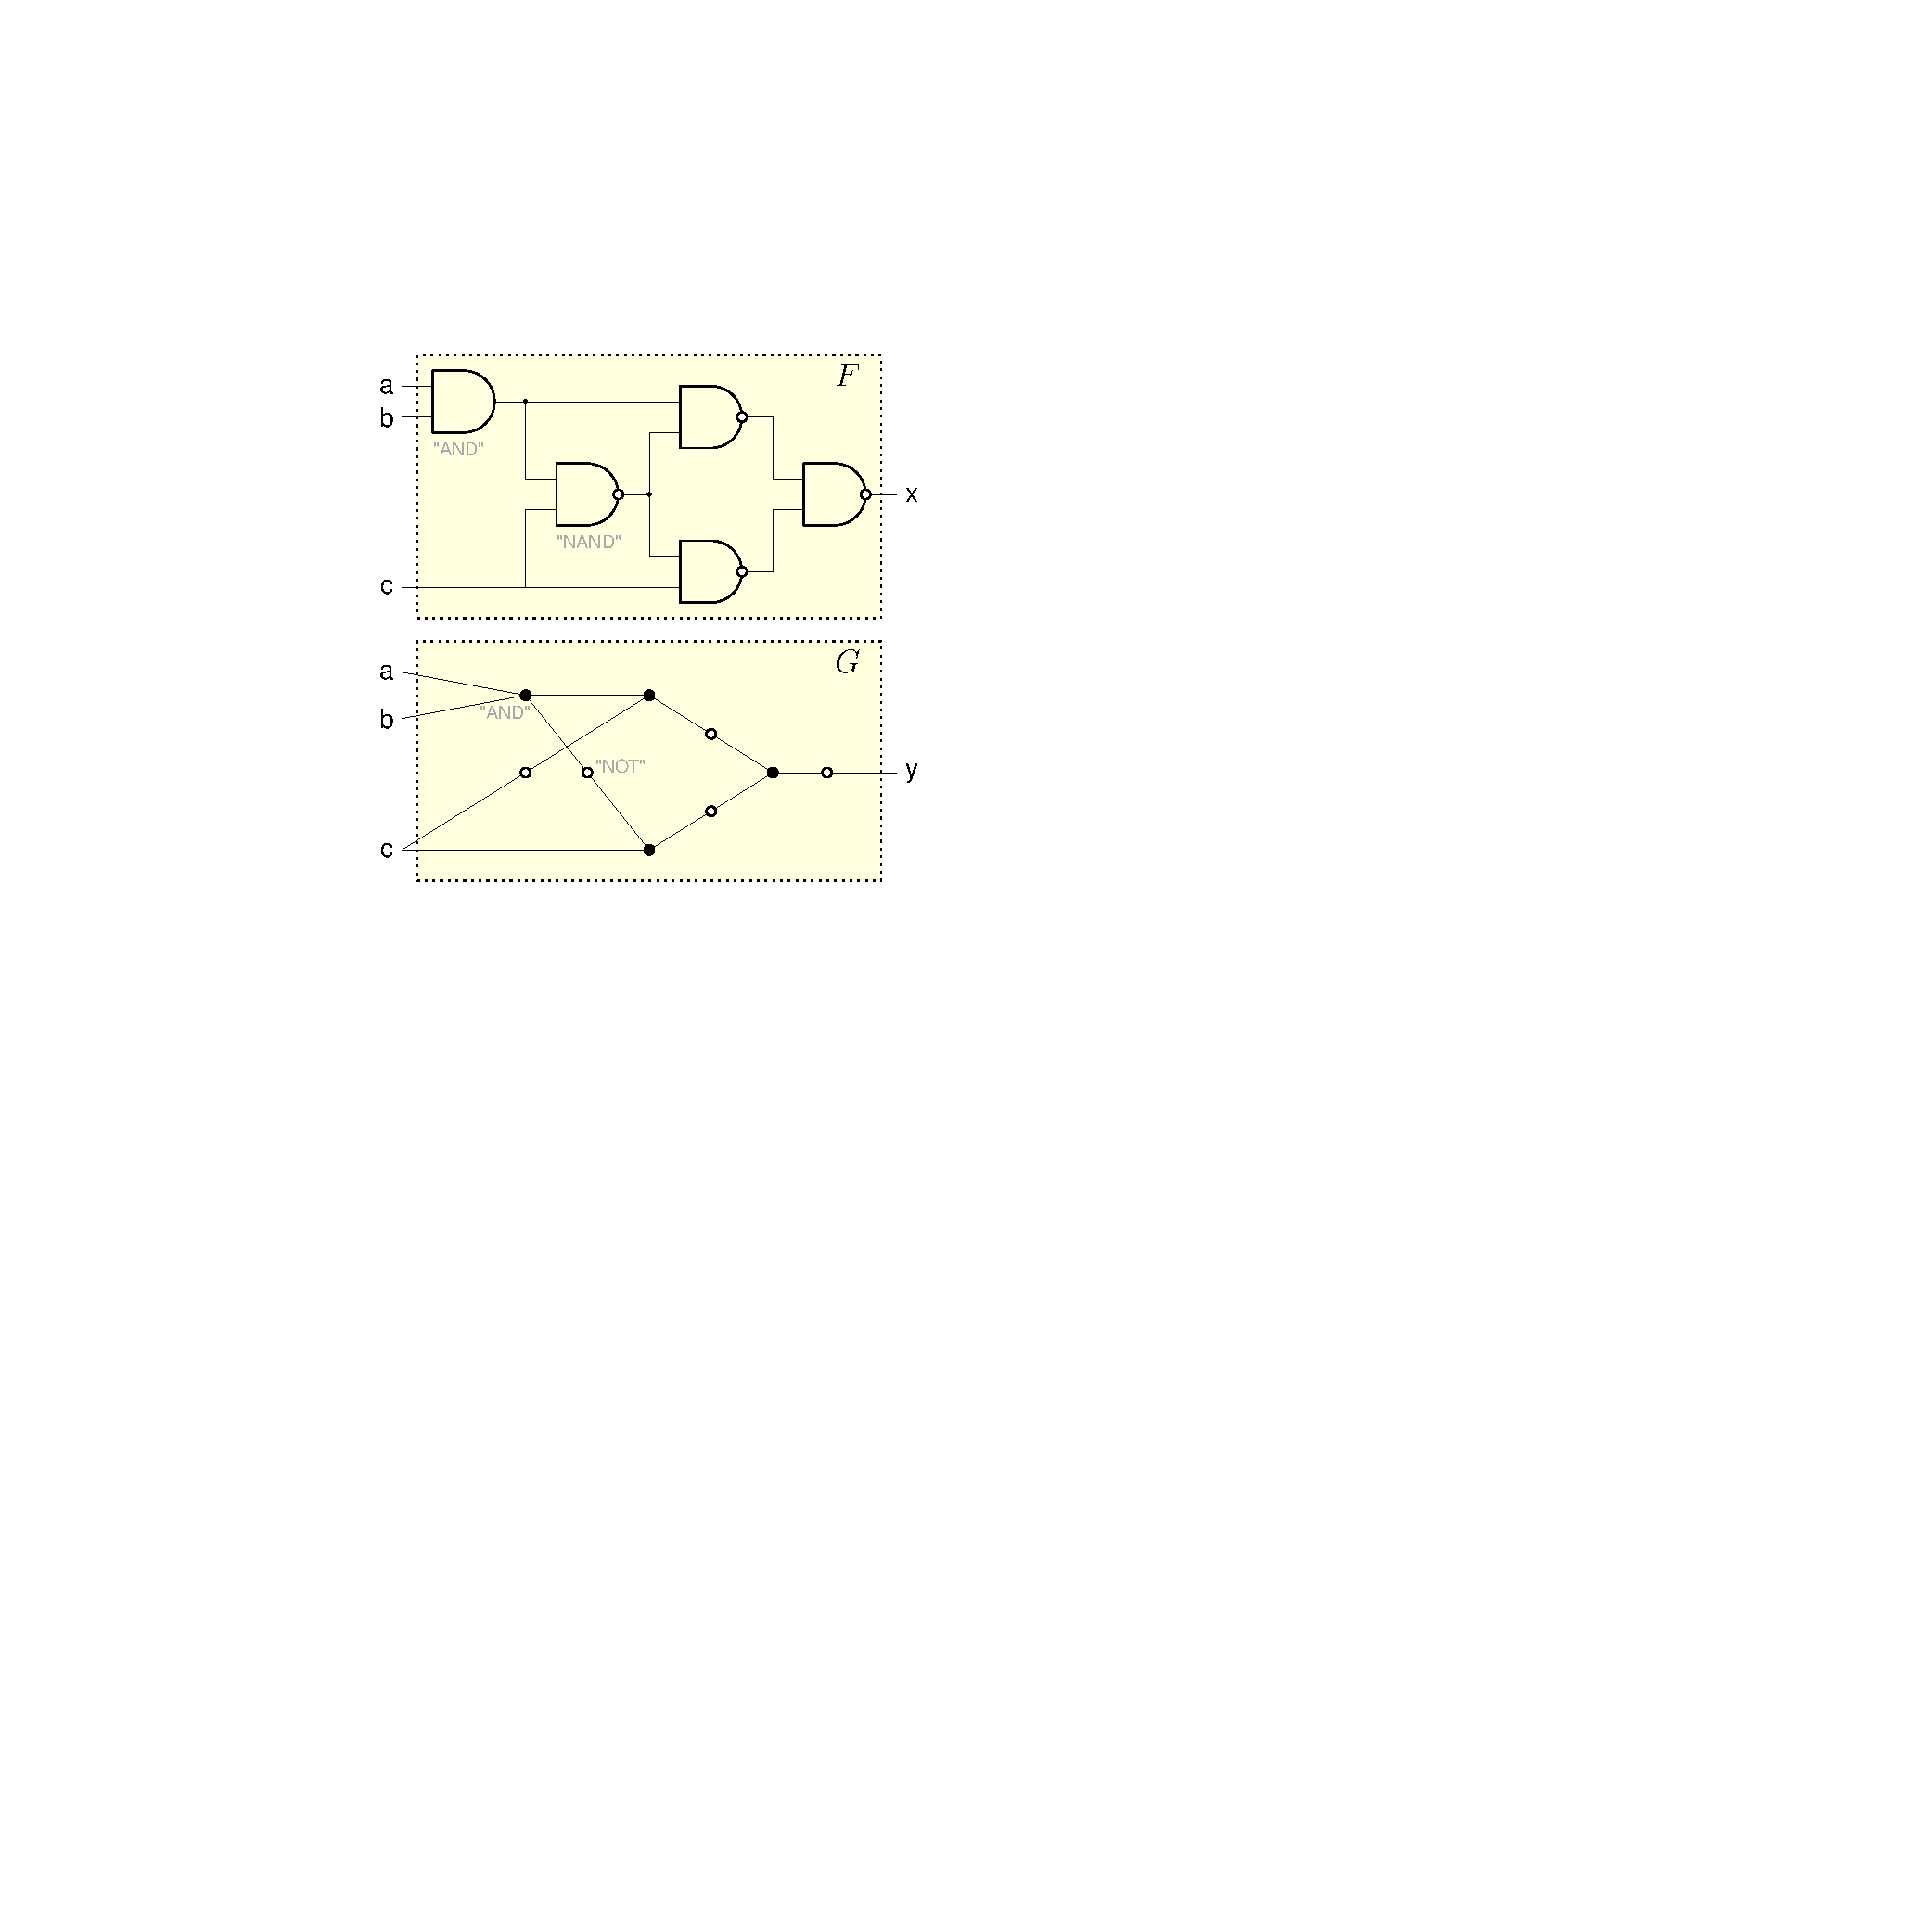
\includegraphics[width=0.8\textwidth,page=1]{figures/l11/circuits-aig.pdf}}%
		\only<3>{\includegraphics[width=0.8\textwidth,page=2]{figures/l11/circuits-aig.pdf}}%
		\only<4>{\includegraphics[width=0.8\textwidth,page=3]{figures/l11/circuits-aig.pdf}}%
		\only<5>{\includegraphics[width=0.8\textwidth,page=4]{figures/l11/circuits-aig.pdf}}%
		\only<6-7>{\includegraphics[width=0.8\textwidth,page=5]{figures/l11/circuits-aig.pdf}}%
		\only<8>{\includegraphics[width=0.8\textwidth,page=6]{figures/l11/circuits-aig.pdf}}%
		\only<9>{\includegraphics[width=0.8\textwidth,page=7]{figures/l11/circuits-aig.pdf}}%
		\only<10>{\includegraphics[width=0.8\textwidth,page=8]{figures/l11/circuits-aig.pdf}}%
		\only<11->{\includegraphics[width=0.8\textwidth,page=9]{figures/l11/circuits-aig.pdf}}%
	\end{minipage}%
\end{frame}

\begin{frame}{CEC: Remarks}
	\begin{itemize}
		\item Important cornerstone of \textbf{Electronic Design Automation}~\cite{marques2000boolean}\\
		-- can be used to validate \highlo{implementation} based on \highl{specification}\\
		-- other EDA techniques: model checking, \highl{Automated Test Pattern Generation (ATPG)}
		\item Crucial ``\highl{intrinsically Boolean}'' benchmark problem throughout history of SAT solving\\
		-- Every SAT competition features miters
		\item SAT sweeping originally proposed for \highl{bounded model checking}~\cite{kuehlmann2004dynamic}
		\item Gate recognition and merging now a form of general inprocessing for \highl{any formula},\\
		connected to variable elimination~\cite{biere2022gimsatul}
	\end{itemize}
\end{frame}

\begin{frame}{Analyzing Cryptographic Building Blocks}
	% http://www.inrialpes.fr/planete/people/ccastel/PAPERS/SAT09.pdf
	% cryptanalysis of ASCON: https://eprint.iacr.org/2015/030.pdf
	\textbf{Cryptanalysis} = analyze, attempt to ``break'' cryptographic building blocks to test, advance them
	\begin{itemize}
		\item Building blocks: Stream ciphers (\ (msg,key) $\mapsto$ encrypted msg \ )~\cite{soos09extending}, \ hash functions~\cite{dobraunig2015cryptanalysis}, \ldots
		\item \highl{Algebraic cryptanalysis}: try to build equations relating output to input~\cite{soos09extending}
		\begin{itemize}
			\item SAT solver should support \highl{XOR clauses}
			\item SAT solver should use \highl{Gaussian Elimination} as a sub-program
		\end{itemize}
		\pause
		\item Established SAT-based approaches:
		\begin{itemize}
			\item Prove mathematical properties of internal states~\cite{dobraunig2015cryptanalysis}
			\item Find weak keys and preimages~\cite{lafitte2014applications}
			\item Find collisions of hash functions~\cite{mironov2006applications}
		\end{itemize}
		\pause
		\item Cross-application use of SAT techniques:
		\begin{itemize}
			\item Cryptanalysis via SMT solving~\cite{xin2019improved}
			\item Cryptanalysis via bounded model checking~\cite{manthey2023testing}
			\item Hash function analysis also used in algorithm design~\cite{weaver2020constructing}
		\end{itemize}
	\end{itemize}
	
	\vspace*{2mm}
	``\textit{\unimp{it turns out that the highly combinatorial nature of the problem is not well suited for linear solvers, and that SAT solvers are a better fit for this type of problem}}'' ---Dobraunig et al.\ after trying MILP for ASCON~\cite{dobraunig2015cryptanalysis}
\end{frame}

\begin{frame}{Multi Agent Path Finding~\cite{surynek2022migrating}}
	% https://www.jair.org/index.php/jair/article/download/13318/26769/
	\begin{minipage}[c][8cm][t]{0.55\textwidth}
		\begin{itemize}
			\item Discretized \highl{2D grid of positions}, $n$ \highl{cooperative agents}
			\item Discretized time steps: move \highl{0-1 cells per time step}
			\item Per agent: Initial position and goal position
			\item<2-> \highlo{Collisions disallowed}
			\item<2-> Optimize \highl{makespan} (= steps until all goals reached)\\
			or \highl{Sum of Costs} (= total number of actions performed)
		\end{itemize}
		\only<7->{
		\begin{block}{Optimal Approaches to MAPF}
			\begin{itemize}
				\item \highl{M$^*$ algorithm}: adjusted $A^*$ with collision handling\\and backtracking
				\item \highl{Conflict Based Search (CBS)}: route individually; at collision, add constraint to a colliding agent and re-route
				\item \highl{Reduction-based approaches}: SAT, MaxSAT, ASP, CSP
			\end{itemize}
		\end{block}
		}
	\end{minipage}%
	\begin{minipage}[c][8cm][t]{0.45\textwidth}
		\hfill%
		\only<1>{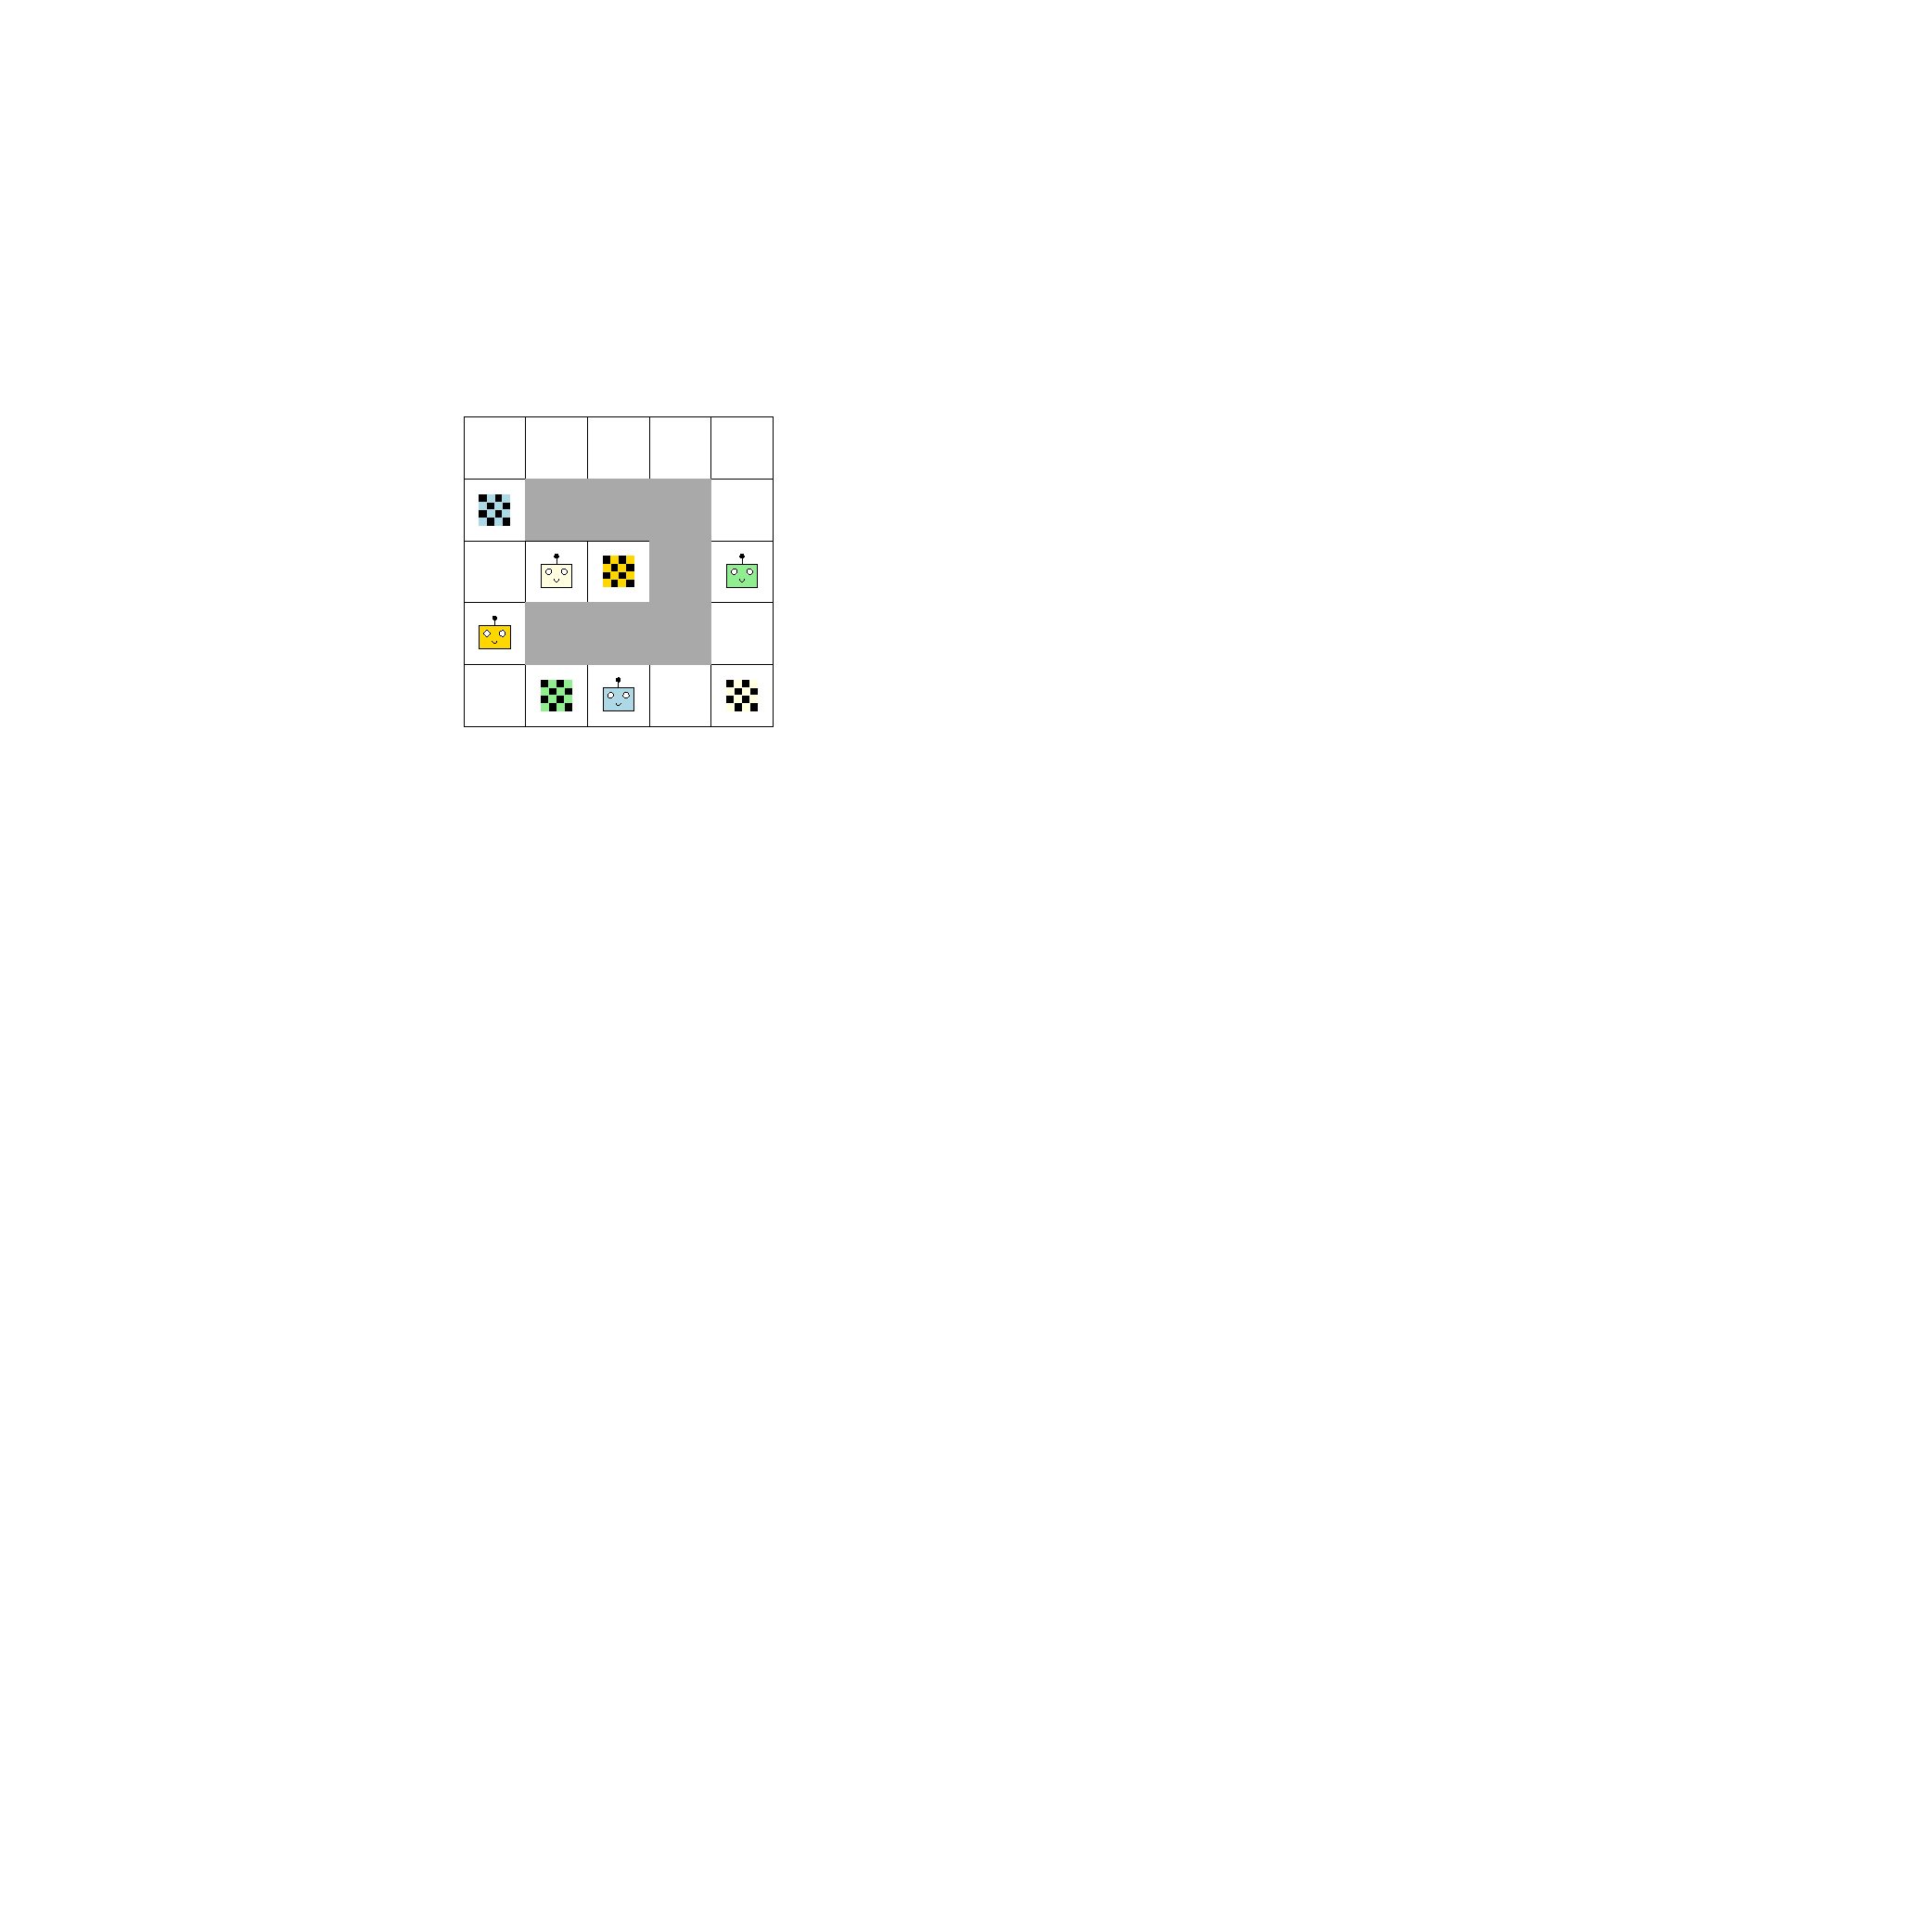
\includegraphics[width=0.9\textwidth,page=1]{figures/l11/mapf.pdf}}%
		\only<2>{\includegraphics[width=0.9\textwidth,page=2]{figures/l11/mapf.pdf}}%
		\only<3>{\includegraphics[width=0.9\textwidth,page=3]{figures/l11/mapf.pdf}}%
		\only<4>{\includegraphics[width=0.9\textwidth,page=4]{figures/l11/mapf.pdf}}%
		\only<5>{\includegraphics[width=0.9\textwidth,page=5]{figures/l11/mapf.pdf}}%
		\only<6->{\includegraphics[width=0.9\textwidth,page=6]{figures/l11/mapf.pdf}}%
	\end{minipage}%
\end{frame}

\begin{frame}{Is SAT-based MAPF worthwhile?}
	\textbf{Observation on MAPF}~\cite{surynek2022migrating} (and planning, and scheduling, and probably many other problems \ldots):\\[4mm]
	\begin{minipage}[c][8cm][t]{0.45\textwidth}
		\textbf{Direct search-based approaches}\\
		perform especially well on \highl{large},\\
		\highlo{lightly constrained} instances.
		\\[0mm]
		
		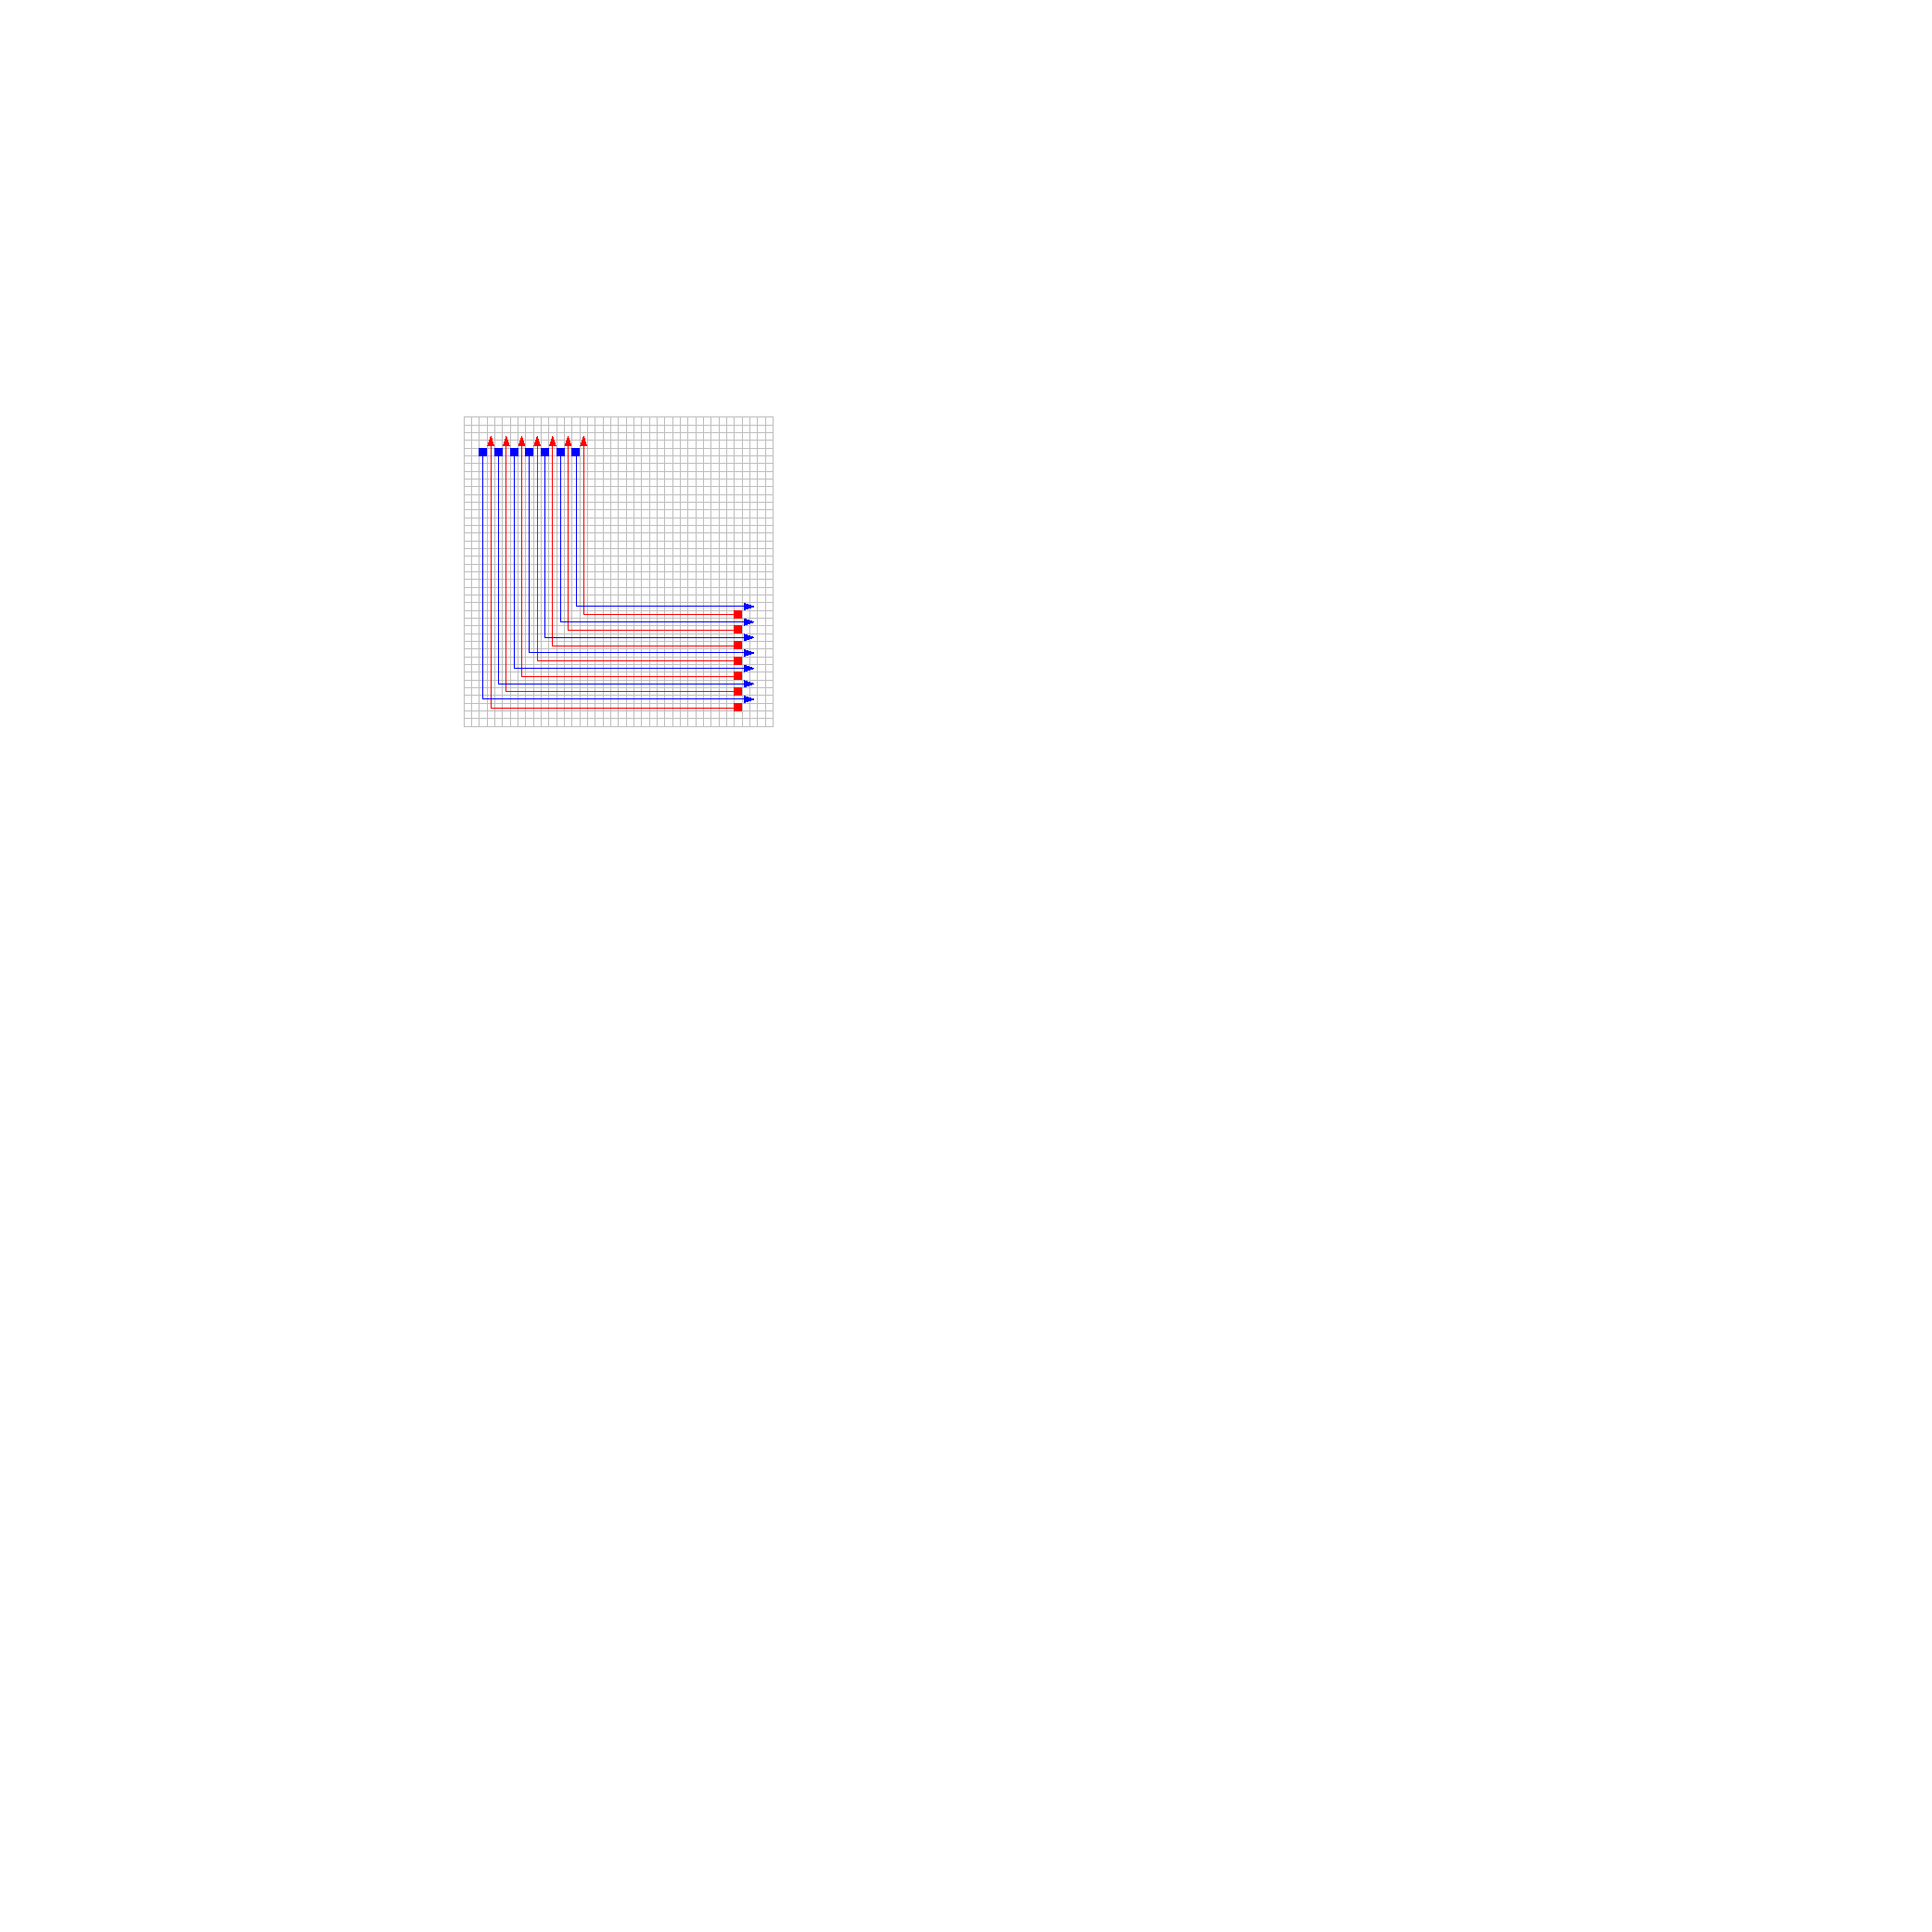
\includegraphics[height=4cm]{figures/l11/mapf-large.pdf}
	\end{minipage}%
	\begin{minipage}[c][8cm][t]{0.1\textwidth}
		\ 
	\end{minipage}%
	\begin{minipage}[c][8cm][t]{0.45\textwidth}
		\textbf{SAT-based approaches}\\
		perform especially well on \highlo{small-sized},\\
		\highl{highly constrained} instances.
		\\[0mm]
		
		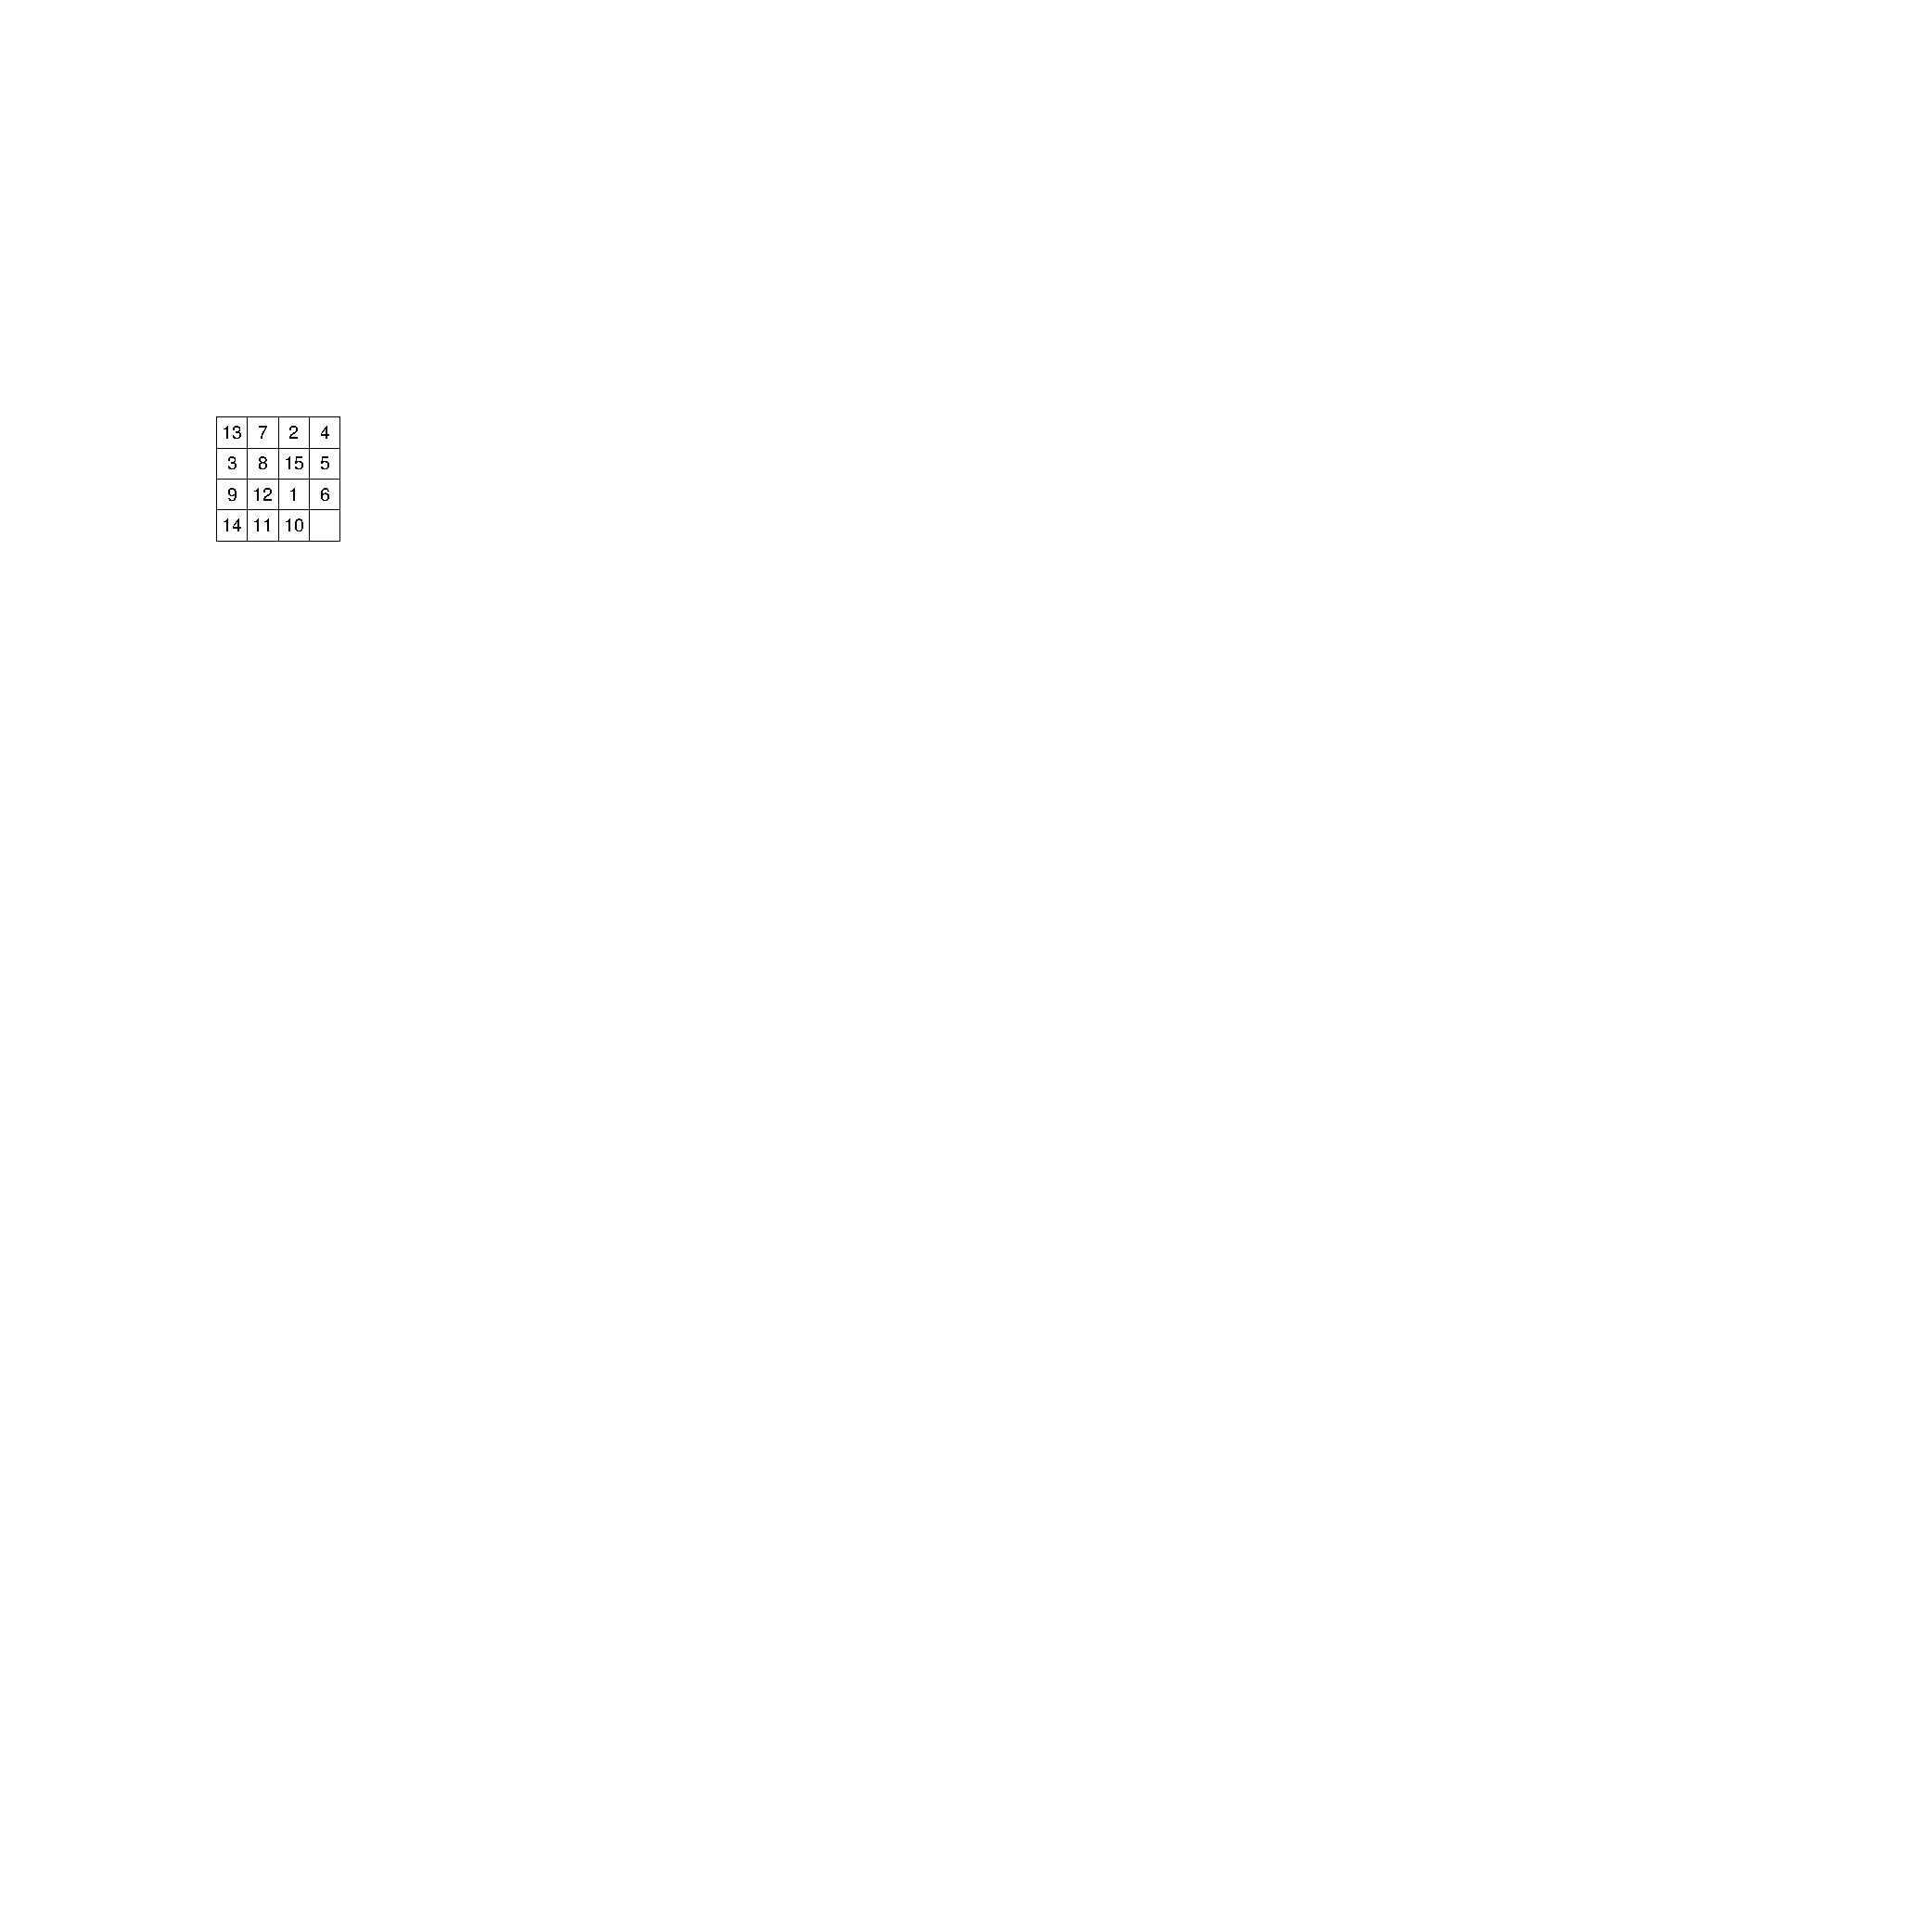
\includegraphics[height=4cm]{figures/l11/mapf-small.pdf}
	\end{minipage}%
\end{frame}

\begin{frame}{Explainable AI: Learning Decision Trees}
% https://ojs.aaai.org/index.php/AAAI/article/download/16509/16316
	\begin{minipage}[c][8cm][t]{0.52\textwidth}
		\begin{itemize}
			\item Given: $n$ $d$-dimensional sample vectors ($d$ \highl{features}) mapped to a \highl{(binary) class}
			\item Task: \highl{Learn decision tree} classifying all samples
			\item \highl{Explainable classifier} (the more shallow the better)
		\end{itemize}
		\only<2>{
		\begin{block}{SAT-based approach~\cite{narodytska2018learning}}
			\begin{itemize}
				\item Encode \highlo{complete binary tree} of depth $k$
				\item Encode recursively for each node which samples are \highl{excluded} along its path
				\item Constrain that \highl{0-leaves exclude all 1-labeled samples} and vice versa
				\item Solver picks a \highl{sub-tree} and \highl{each node's feature}
			\end{itemize}
		\end{block}
		}
	\end{minipage}%
	\begin{minipage}[c][8cm][t]{0.03\textwidth}
		\ 
	\end{minipage}%
	\begin{minipage}[c][8cm][t]{0.45\textwidth}
		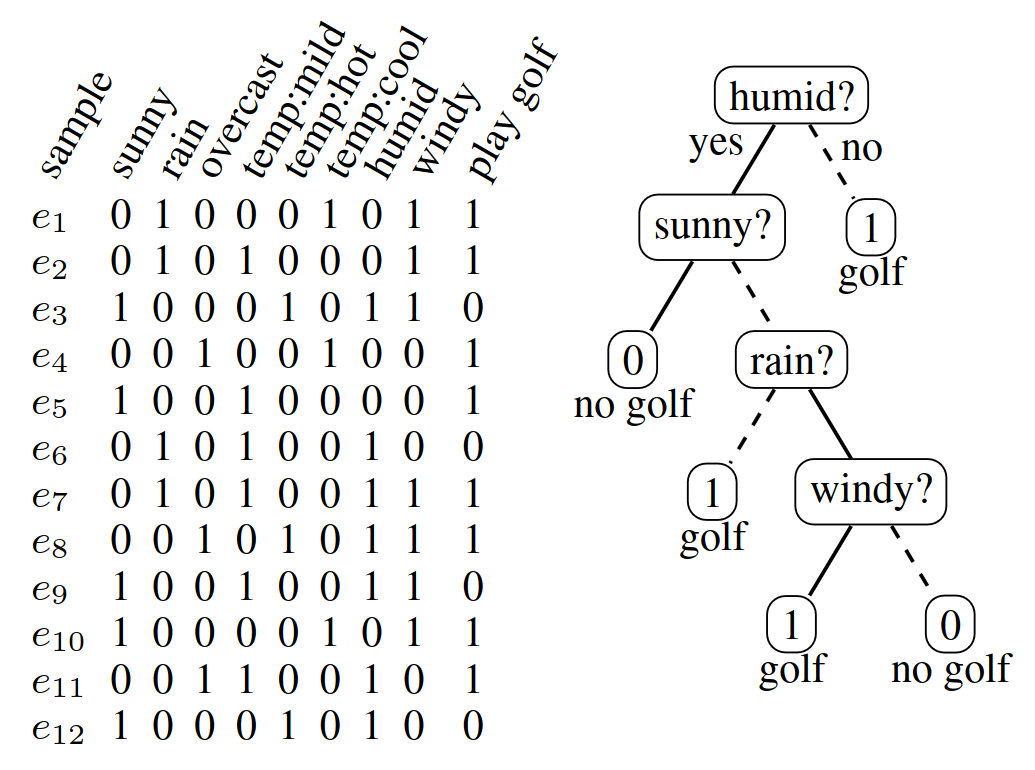
\includegraphics[width=\textwidth]{figures/l11/decisiontree.png}
		
		\hfill\unimp{\small{}taken from \cite{schidler2021sat}}
		%\uncover<2->{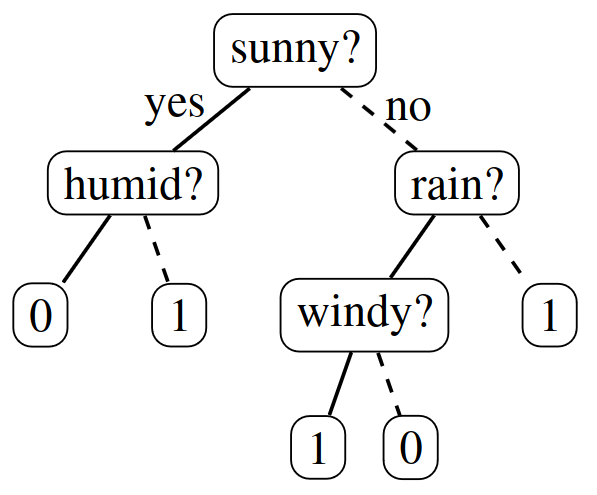
\includegraphics[width=0.35\textwidth]{figures/l11/decisiontree-smaller.png}}\\
	\end{minipage}%
\end{frame}

\begin{frame}{SAT-based Improvement of Decision Trees~\cite{schidler2021sat}}
	\begin{itemize}
		\item SAT-based approach \highlo{slow/infeasible} for large data sets
		\item Better: Construct \highlo{initial decision tree heuristically}, then \highl{locally improve sub-trees via SAT}
		\begin{itemize}
			\item \textbf{Hybrid approach}, also beneficial in other contexts, e.g., CEC, planning~\cite{froleyks2019pasar}
		\end{itemize}
		\item Enables to scale up merits of SAT to \highl{arbitrarily large data sets}
	\end{itemize}
	\begin{center}
		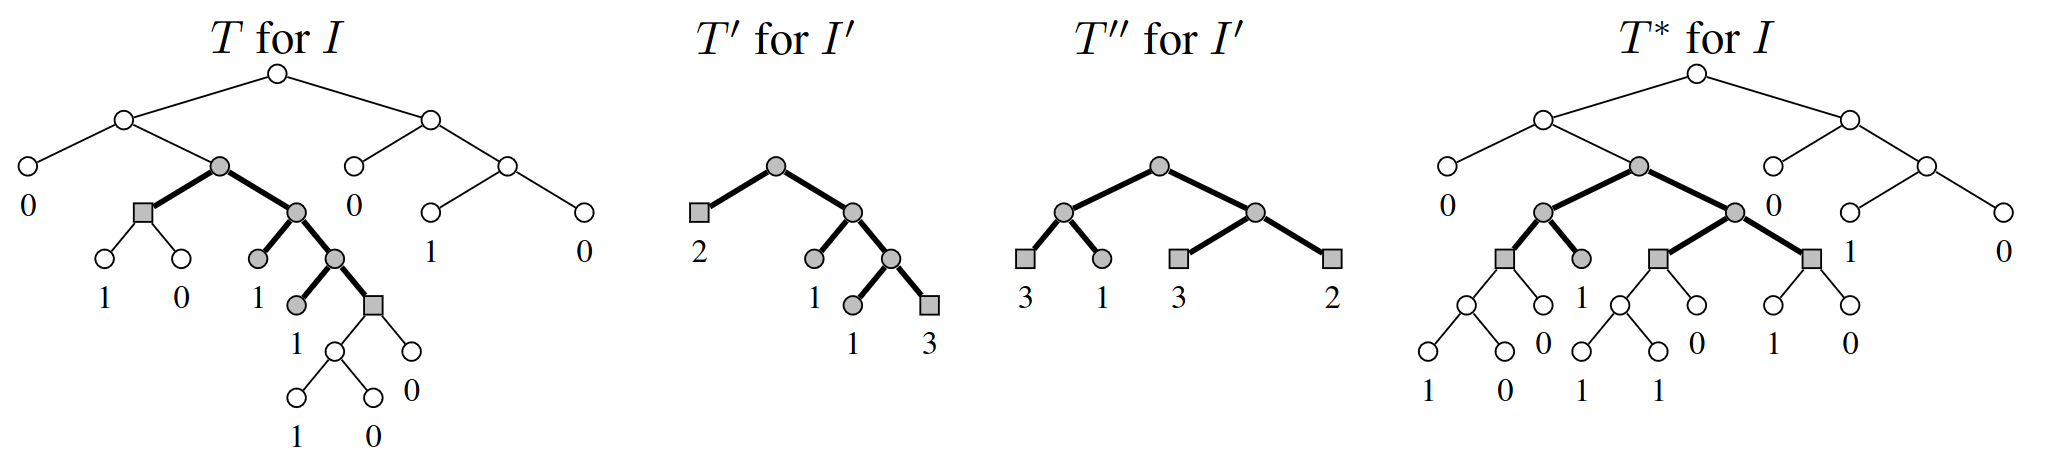
\includegraphics[width=0.95\textwidth]{figures/l11/decisiontree-improvement.png}
		
		\hfill\unimp{\small{}taken from \cite{schidler2021sat}}
	\end{center}
\end{frame}

\begin{frame}{More on SAT Solving $\times$ Machine Learning}
	\vspace*{-3mm}
	\begin{itemize}
		\item \highl{Algorithm selection}\\
		\unimp{\small{}Xu, Lin, et al. ``SATzilla: portfolio-based algorithm selection for SAT.'' JAIR 2008.}\\
		\unimp{\small{}Eggensperger, Katharina, Marius Lindauer, and Frank Hutter. ``Neural networks for predicting algorithm runtime distributions.'' IJCAI 2018.}
		\vspace*{2mm}
		\item SAT Solving \highl{featuring ML techniques}\\
		\unimp{\small{}Liang, Jia Hui, et al. ``Learning rate based branching heuristic for SAT solvers.'' SAT 2016.}\\
		\unimp{\small{}Guo, Wenxuan, et al. ``Machine learning methods in solving the boolean satisfiability problem.'' Machine Intelligence Research (2023).}
		\vspace*{2mm}
		\item \highl{Verify Neural Networks} via SAT/SMT solving\\
		\unimp{\small{}Huang, Xiaowei, et al. ``Safety verification of deep neural networks.'' CAV 2017.}\\
		\unimp{\small{}Ehlers, Ruediger. ``Formal verification of piece-wise linear feed-forward neural networks.'' ATVA 2017.}
		\vspace*{2mm}
		\item \highl{Analyze and understand} behavior of SAT solvers and instances\\
		\unimp{\small{}Soos, Mate, Raghav Kulkarni, and Kuldeep S. Meel. ``CrystalBall: gazing in the black box of SAT solving.'' SAT 2019.}\\
		\unimp{\small{}Fuchs, Tobias, Jakob Bach, and Markus Iser. ``Active Learning for SAT Solver Benchmarking.'' TACAS 2023.}
	\end{itemize}
\end{frame}

\begin{frame}{Train Scheduling with Disruptions via MaxSAT~\cite{lemos2024iterative}}
	% https://jair.org/index.php/jair/article/view/14924/27025
	\only<1-3>{
	\centering
	\vspace*{2cm}
	\uncover<1->{\textbf{Can SAT Solving fix the Deutsche Bahn?}}
	\\\uncover<2->{No.}
	\\\uncover<3->{But it might make the Swiss trains run even better!}
	}%
	\only<4->{
	\begin{minipage}[c][8cm][t]{0.45\textwidth}
		\vspace*{-1mm}
		\textbf{Train Scheduling Optimization Problem} (TSOP)%
		\begin{itemize}
			\item \highl{Route} trains through predefined stations
			\item \highl{Schedule} train timetable subject to time\\
			and resource constraints
		\end{itemize}
		\uncover<5->{
		\textbf{TSOP Under Disruption} (TSOPUD)
		\begin{itemize}
			\item Numerous \highlo{disruptions}: slowdown, train blocked, track blocked, staffing / rolling stock
			\item Reroute, reschedule to \highl{minimize delays}
		\end{itemize}
		}
		\uncover<6->{
		\vspace*{-1mm}
		\begin{block}{MaxSAT-based approach}
			\begin{itemize}
				\item Encode time requirements as hard clauses,\\
				route/train cost as \highl{soft clauses}
				\item \highl{Relax timings incrementally} until feasible
				\item \highlo{Add disruption(s)}, \highl{relax timings} as needed
			\end{itemize}
		\end{block}	
		}
	\end{minipage}%
	\begin{minipage}[c][8cm][t]{0.03\textwidth}
		\ 
	\end{minipage}%
	\begin{minipage}[c][8cm][t]{0.52\textwidth}
		\vspace*{-2mm}
		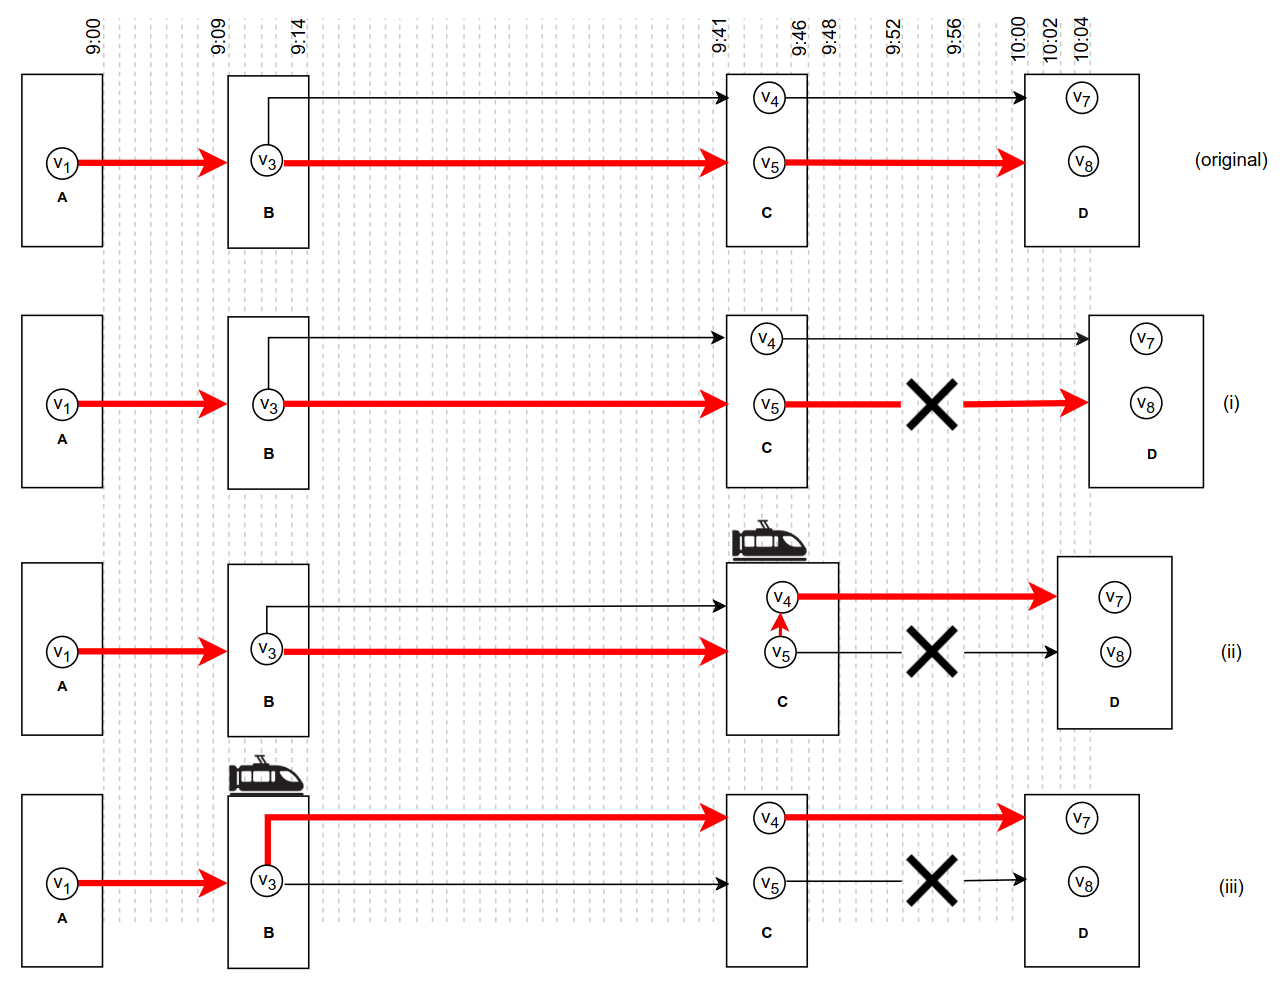
\includegraphics[width=\textwidth]{figures/l11/train-scheduling.png}
		
		\vspace*{-2mm}
		\hfill\unimp{\small{}taken from \cite{lemos2024iterative}}
	\end{minipage}%
	}
\end{frame}

\begin{frame}{Application Highlights: Takeaways}
	\vspace*{-3mm}
	\begin{itemize}
		\item SAT is an (actually!) \highl{\textbf{essential and well-established tool}} for
		\begin{itemize}
			\item software \& hardware verification
			\item electronic design automation
			\item specific cryptanalysis tasks.
		\end{itemize}
		\item Indicators for a problem to best use SAT for?
		\begin{itemize}
			\item large portion of ``\highl{intrinsically Boolean}'' constraints
			\item \highl{combinatorial search space} / set of decisions, \highlo{NP-hard (or harder)}
			\item problem description \highlo{not too large}
		\end{itemize}
		\item \highl{Cross-application} techniques and insights:
		\begin{itemize}
			\item Often promising to \highl{hybridize} SAT with direct (search) methods: use SAT to resolve \highlo{difficult cores}
			\item \highl{Positive feedback loop} between solver techniques and applications
			\item \highl{Cross-fertilization} between different applications (e.g., BMC, SMT)
		\end{itemize}
		\item \textbf{Many more}, sometimes important, \textbf{applications} of SAT we didn't talk about
		\begin{itemize}
			\item Automated test pattern generation, graph theory, theorem proving, social choice theory, puzzle solving, knowledge compilation, combinatorial design theory, \ldots
		\end{itemize}
	\end{itemize}
\end{frame}

\begin{frame}[allowframebreaks]{References}
	\renewcommand*{\bibfont}{\scriptsize}
	\printbibliography
\end{frame}

\end{document}
